\documentclass[a4paper,10.5pt]{ltjsarticle}
\usepackage{graphicx}
\usepackage{luatexja-fontspec}
\usepackage{caption}
\usepackage{amsmath,amssymb,bm,braket}
\usepackage{gnuplot-lua-tikz}
\usepackage[top=10truemm,bottom=15truemm,left=10truemm,right=10truemm]{geometry}
\usepackage{array}
\usepackage{upgreek}
\usepackage{fancyhdr}
\renewcommand{\refname}{}
\usepackage{listings,jvlisting}
\usepackage{tikz}
\usetikzlibrary{external}
\tikzexternalize
\lstset{
  basicstyle={\ttfamily},
  identifierstyle={\small},
  commentstyle={\smallitshape},
  keywordstyle={\small\bfseries},
  ndkeywordstyle={\small},
  stringstyle={\small\ttfamily},
  frame={tb},
  breaklines=true,
  columns=[l]{fullflexible},
  numbers=left,
  xrightmargin=0pt,
  xleftmargin=3pt,
  numberstyle={\scriptsize},
  stepnumber=1,
  numbersep=1pt,
  lineskip=-0.5ex
}
\captionsetup[figure]{format=plain, labelformat=simple, labelsep=quad,labelfont=bf}
\captionsetup[table]{format=plain, labelformat=simple, labelsep=quad,labelfont=bf}
\parindent = 0pt
\setmainjfont[BoldFont=HiraMinProN-W6]{HiraMinPro-W3}
%[BoldFont=HGSMinchoE]{MSMincho}[BoldFont=HiraMinProN-W6]{HiraMinPro-W3}
\begin{document}
\centerline{\HUGE \bfseries 物理情報工学CD実験 報告書}
\centerline{ }
\rightline{\vspace{-3mm} \Large 2023年度   }
\begin{table}[h]
  \newcolumntype{I}{!{\vrule width 1.5pt}}
  \newcolumntype{i}{!{\vrule width 0.8pt}}
  \arrayrulewidth=0.8pt
  \renewcommand{\arraystretch}{1.5}
  \newcommand{\bhline}[1]{\noalign{\hrule height #1}}
  \huge
  \centering
  \begin{tabular}{Iwc{6cm}Iwc{2cm}iciwc{5cm}I}
    \bhline{1.5pt}
    実験テーマ&\multicolumn{3}{cI}{D4\ AD/DA変換回路}\\
    \hline
    担当教員名&\multicolumn{3}{cI}{増田}\\
    \hline
    実験整理番号&80&実験者氏名&平井 優我\\
    \hline
    共同実験者氏名&\multicolumn{3}{cI}{藤井\ 大樹}\\
    \hline
    曜日組&木&実験日&12月14日\\
    \hline
    実験回&8&報告書提出日&12月20日\\
    \bhline{1.5pt}
  \end{tabular}
\end{table}
\clearpage
%1-2-------------------------------------------------------------------------
\hspace{-2pt}{\Large \bfseries 1.目的}\\
 デジタル信号の特徴を理解すると共に、アナログ信号のデジタル処理に必要なアナログ・デジタル変換の方法と性質を、実験を通じて理解する。\\
\\
\hspace{-2pt}{\Large \bfseries 2.結果と考察}\\
{\large \bfseries 2.1 実験1}\\
 図\ref{A_D}にサンプルホールド波形(緑)、図\ref{D_A}にLPF通過波形(緑)を示す。ただし、黄色の波形は入力正弦波を表す。
\begin{figure}[h]
  \centering
  \begin{minipage}[h]{0.45\linewidth}
    \includegraphics[scale=0.18]{JOUON01.eps}
    \caption*{(a)}
  \end{minipage}
  \begin{minipage}[h]{0.43\linewidth}
    \includegraphics[scale=0.18]{JOUON02.eps}
    \caption*{(b)}
  \end{minipage}
  \begin{minipage}[h]{0.45\linewidth}
    \includegraphics[scale=0.18]{JOUON03.eps}
    \caption*{(c)}
  \end{minipage}
  \begin{minipage}[h]{0.43\linewidth}
    \includegraphics[scale=0.18]{JOUON04.eps}
    \caption*{(d)}
  \end{minipage}
  \caption{アナログ波形をデジタル波形にしたグラフ\ サンプリング周波数(a)$10\ \mathrm{kHz}$\ (b)$5\ \mathrm{kHz}$\ (c)$2\ \mathrm{kHz}$\ (d)$1\ \mathrm{kHz}$}
  \label{A_D}
\end{figure}\\
図\ref{A_D}から、サンプリング周波数を大きくすればするほどサンプルホールド波形は入力正弦波に近い形となった。また、サンプルホールド波形は入力正弦波と位相が一致した。そして、サンプルホールド波形は値が一定となるような部分の数が周波数に比例して変化しているため妥当な形となった。
\clearpage
\begin{figure}[h]
  \centering
  \begin{minipage}[h]{0.45\linewidth}
    \includegraphics[scale=0.18]{JOUON05.eps}
    \caption*{(a)}
  \end{minipage}
  \begin{minipage}[h]{0.43\linewidth}
    \includegraphics[scale=0.18]{JOUON06.eps}
    \caption*{(b)}
  \end{minipage}
  \begin{minipage}[h]{0.45\linewidth}
    \includegraphics[scale=0.18]{JOUON07.eps}
    \caption*{(c)}
  \end{minipage}
  \begin{minipage}[h]{0.43\linewidth}
    \includegraphics[scale=0.18]{JOUON08.eps}
    \caption*{(d)}
  \end{minipage}
  \caption{デジタル波形をアナログ波形にしたグラフ\ サンプリング周波数(a)$10\ \mathrm{kHz}$\ (b)$5\ \mathrm{kHz}$\ (c)$2\ \mathrm{kHz}$\ (d)$1\ \mathrm{kHz}$}
  \label{D_A}
\end{figure}
図\ref{D_A}から、サンプリング周波数が$10,5,2\ \mathrm{kHz}$のとき、LPF通過波形は入力正弦波に近い形となった。これより、アナログ波形の周波数$1\ \mathrm{kHz}$の2倍以上のサンプリング周波数だと、LPF通過波形が入力正弦に近い形となり、サンプリング定理が成り立っている。また、LPF通過波形は入力波形よりも位相が早くなった。そして、LPF通過波形はサンプルホールド波形の急激に値が変化した部分をなめらかにしたような波形となった。\\
 周波数を連続的に変化させたときにサンプルホールド波形とLPF通過波形がどのように変化するかを考える。まず、サンプルホールド波形について、周波数を大きくすると値が一定となる部分が小さくなり入力正弦波に近づいていくと考えられる。逆に周波数を小さくするとき、入力波形をそのままサンプリングする部分とその値をホールドする部分が長くなっていき、元の入力波形と一定値が交互に繰り返されるような波形となる。\\
 図\ref{A_D}について、振幅の減衰と位相差を見積もると表\ref{ADattenuation-delay}となる。
\begin{table}[h]
  \newcolumntype{I}{!{\vrule width 1.5pt}}
  \newcolumntype{i}{!{\vrule width 0.5pt}}
  \arrayrulewidth=0.8pt
  \renewcommand{\arraystretch}{1.5}
  \newcommand{\bhline}[1]{\noalign{\hrule height #1}}
  \centering
  \caption{振れ幅の減衰と位相差}
  \label{ADattenuation-delay}
  \begin{tabular}{IciccI}
    \bhline{1.5pt}
    \begin{tabular}{c}
      サンプリング\\[-10pt]
      周波数\ /\ kHz\\
    \end{tabular}
    &振幅の減衰率&位相差\\
    \hline
    10&0.99&$-0.012$\pi\\
    5&1.0&$-0.011\pi$\\
    2&0.86&$-0.0035\pi$\\
    1&0.88&$0.0\pi$\\
    \bhline{1.5pt}
  \end{tabular}
\end{table}
\clearpage
表\ref{ADattenuation-delay}から、サンプリング周波数が5\ kHzよりも小さくなると振幅が減衰することがわかる。これは入力波形の周波数に対してサンプリング周波数が小さく、入力波形で最大振幅が実現される直前の領域で値がホールドされていることに起因する。ただし、サンプリングする位相をずらすことで振幅の減衰率は1になり得る。\\
 次に、図\ref{D_A}について、振幅の減衰と位相差を見積もると表\ref{DAattenuation-delay}となる。
\begin{table}[h]
  \newcolumntype{I}{!{\vrule width 1.5pt}}
  \newcolumntype{i}{!{\vrule width 0.5pt}}
  \arrayrulewidth=0.8pt
  \renewcommand{\arraystretch}{1.5}
  \newcommand{\bhline}[1]{\noalign{\hrule height #1}}
  \centering
  \caption{振れ幅の減衰と位相差}
  \label{DAattenuation-delay}
  \begin{tabular}{IciccI}
    \bhline{1.5pt}
    \begin{tabular}{c}
      サンプリング\\[-10pt]
      周波数\ /\ kHz\\
    \end{tabular}
    &振幅の減衰率&位相差\\
    \hline
    10&0.49&$-0.54\pi$\\
    5&0.49&$-0.54\pi$\\
    2&0.50&$-0.50\pi$\\
    1&0.47&$-0.64\pi$\\
    \bhline{1.5pt}
  \end{tabular}
\end{table}\\
 表\ref{DAattenuation-delay}から、振幅の減衰率はサンプリング周波数によらず約$-6$\ dBなり、位相差はサンプリング周波数によらず約$\pi/2$となった。これらの結果から位相差も振幅の減衰も理論値とほぼ一致し、表\ref{DAattenuation-delay}の結果は妥当である。\\
 次にFGによって発生される正弦波とパルス波のタイミングのずれについて考える。正弦波とパルス波のタイミングがずれると、サンプルホールドするタイミングがずれることは自明である。これにより、正弦波の山または谷の直前でホールドすればサンプルホールド波形の振幅は小さくなる。逆に、正弦波の山または谷の直後でホールドすればサンプルホールド波形の振幅は入力正弦波に一致する。\\
\\
{\large \bfseries 2.2 実験2}\\
{\large \bfseries 2.2.1\ DA変換}\\
 図\ref{DA}に入力と出力の関係を示す。ただし、点は測定値、黒線は測定点を直線で繋いだ線、赤の破線は原点と$(256,5)$を繋ぐ直線を表す。\\
\begin{figure}[h]
  \centering
  \scalebox{0.7}[0.7]{
\begin{tikzpicture}[gnuplot]
%% generated with GNUPLOT 5.4p10 (Lua 5.4; terminal rev. Jun 2020, script rev. 118)
%% Wed Dec 13 23:10:21 2023
\path (0.000,0.000) rectangle (12.500,8.750);
\gpcolor{color=gp lt color border}
\gpsetlinetype{gp lt border}
\gpsetdashtype{gp dt solid}
\gpsetlinewidth{1.00}
\draw[gp path] (0.018,0.031)--(0.198,0.031);
\node[gp node right] at (-0.166,0.031) {$0$};
\draw[gp path] (0.018,1.768)--(0.198,1.768);
\node[gp node right] at (-0.166,1.768) {$1$};
\draw[gp path] (0.018,3.506)--(0.198,3.506);
\node[gp node right] at (-0.166,3.506) {$2$};
\draw[gp path] (0.018,5.243)--(0.198,5.243);
\node[gp node right] at (-0.166,5.243) {$3$};
\draw[gp path] (0.018,6.981)--(0.198,6.981);
\node[gp node right] at (-0.166,6.981) {$4$};
\draw[gp path] (0.018,8.718)--(0.198,8.718);
\node[gp node right] at (-0.166,8.718) {$5$};
\draw[gp path] (0.018,0.031)--(0.018,0.211);
\node[gp node center] at (0.018,-0.277) {$0$};
\draw[gp path] (2.452,0.031)--(2.452,0.211);
\node[gp node center] at (2.452,-0.277) {$50$};
\draw[gp path] (4.886,0.031)--(4.886,0.211);
\node[gp node center] at (4.886,-0.277) {$100$};
\draw[gp path] (7.320,0.031)--(7.320,0.211);
\node[gp node center] at (7.320,-0.277) {$150$};
\draw[gp path] (9.754,0.031)--(9.754,0.211);
\node[gp node center] at (9.754,-0.277) {$200$};
\draw[gp path] (12.188,0.031)--(12.188,0.211);
\node[gp node center] at (12.188,-0.277) {$250$};
\draw[gp path] (0.018,8.718)--(0.018,0.031)--(12.480,0.031)--(12.480,8.718)--cycle;
\node[gp node center,rotate=-270,font={\fontsize{17.0pt}{20.4pt}\selectfont}] at (-0.918,4.374) {出力されたアナログ電圧$\ y\ /\ \mathrm{V}$};
\node[gp node center,font={\fontsize{17.0pt}{20.4pt}\selectfont}] at (6.249,-1.046) {入力したデジタル値};
\gpcolor{rgb color={0.000,0.000,0.000}}
\gpsetlinewidth{3.00}
\draw[gp path] (0.018,0.033)--(0.261,0.226)--(0.505,0.301)--(0.748,0.484)--(0.992,0.693)%
  --(1.235,0.844)--(1.478,0.957)--(1.722,1.079)--(1.965,1.298)--(2.209,1.459)--(2.452,1.565)%
  --(2.695,1.699)--(2.939,1.963)--(3.182,2.090)--(3.426,2.189)--(3.669,2.295)--(3.912,2.573)%
  --(4.156,2.663)--(4.399,2.800)--(4.643,2.962)--(4.886,3.158)--(5.129,3.257)--(5.373,3.414)%
  --(5.616,3.539)--(5.860,3.848)--(6.103,4.029)--(6.346,4.244)--(6.590,4.209)--(6.833,4.454)%
  --(7.077,4.541)--(7.320,4.672)--(7.563,4.765)--(7.807,5.167)--(8.050,5.120)--(8.294,5.306)%
  --(8.537,5.396)--(8.780,5.674)--(9.024,5.785)--(9.267,6.032)--(9.511,6.134)--(9.754,6.381)%
  --(9.997,6.435)--(10.241,6.690)--(10.484,6.649)--(10.728,7.052)--(10.971,7.135)--(11.214,7.281)%
  --(11.458,7.316)--(11.701,7.846)--(11.945,7.818)--(12.188,8.129)--(12.431,8.325);
\gpsetpointsize{3.20}
\gp3point{gp mark 7}{}{(0.018,0.033)}
\gp3point{gp mark 7}{}{(0.261,0.226)}
\gp3point{gp mark 7}{}{(0.505,0.301)}
\gp3point{gp mark 7}{}{(0.748,0.484)}
\gp3point{gp mark 7}{}{(0.992,0.693)}
\gp3point{gp mark 7}{}{(1.235,0.844)}
\gp3point{gp mark 7}{}{(1.478,0.957)}
\gp3point{gp mark 7}{}{(1.722,1.079)}
\gp3point{gp mark 7}{}{(1.965,1.298)}
\gp3point{gp mark 7}{}{(2.209,1.459)}
\gp3point{gp mark 7}{}{(2.452,1.565)}
\gp3point{gp mark 7}{}{(2.695,1.699)}
\gp3point{gp mark 7}{}{(2.939,1.963)}
\gp3point{gp mark 7}{}{(3.182,2.090)}
\gp3point{gp mark 7}{}{(3.426,2.189)}
\gp3point{gp mark 7}{}{(3.669,2.295)}
\gp3point{gp mark 7}{}{(3.912,2.573)}
\gp3point{gp mark 7}{}{(4.156,2.663)}
\gp3point{gp mark 7}{}{(4.399,2.800)}
\gp3point{gp mark 7}{}{(4.643,2.962)}
\gp3point{gp mark 7}{}{(4.886,3.158)}
\gp3point{gp mark 7}{}{(5.129,3.257)}
\gp3point{gp mark 7}{}{(5.373,3.414)}
\gp3point{gp mark 7}{}{(5.616,3.539)}
\gp3point{gp mark 7}{}{(5.860,3.848)}
\gp3point{gp mark 7}{}{(6.103,4.029)}
\gp3point{gp mark 7}{}{(6.346,4.244)}
\gp3point{gp mark 7}{}{(6.590,4.209)}
\gp3point{gp mark 7}{}{(6.833,4.454)}
\gp3point{gp mark 7}{}{(7.077,4.541)}
\gp3point{gp mark 7}{}{(7.320,4.672)}
\gp3point{gp mark 7}{}{(7.563,4.765)}
\gp3point{gp mark 7}{}{(7.807,5.167)}
\gp3point{gp mark 7}{}{(8.050,5.120)}
\gp3point{gp mark 7}{}{(8.294,5.306)}
\gp3point{gp mark 7}{}{(8.537,5.396)}
\gp3point{gp mark 7}{}{(8.780,5.674)}
\gp3point{gp mark 7}{}{(9.024,5.785)}
\gp3point{gp mark 7}{}{(9.267,6.032)}
\gp3point{gp mark 7}{}{(9.511,6.134)}
\gp3point{gp mark 7}{}{(9.754,6.381)}
\gp3point{gp mark 7}{}{(9.997,6.435)}
\gp3point{gp mark 7}{}{(10.241,6.690)}
\gp3point{gp mark 7}{}{(10.484,6.649)}
\gp3point{gp mark 7}{}{(10.728,7.052)}
\gp3point{gp mark 7}{}{(10.971,7.135)}
\gp3point{gp mark 7}{}{(11.214,7.281)}
\gp3point{gp mark 7}{}{(11.458,7.316)}
\gp3point{gp mark 7}{}{(11.701,7.846)}
\gp3point{gp mark 7}{}{(11.945,7.818)}
\gp3point{gp mark 7}{}{(12.188,8.129)}
\gp3point{gp mark 7}{}{(12.431,8.325)}
\gpcolor{rgb color={1.000,0.000,0.000}}
\gpsetdashtype{dash pattern=on 5.00*\gpdashlength off 3.00*\gpdashlength }
\draw[gp path] (0.018,0.031)--(0.144,0.119)--(0.270,0.206)--(0.396,0.294)--(0.522,0.382)%
  --(0.647,0.470)--(0.773,0.557)--(0.899,0.645)--(1.025,0.733)--(1.151,0.821)--(1.277,0.908)%
  --(1.403,0.996)--(1.529,1.084)--(1.654,1.172)--(1.780,1.259)--(1.906,1.347)--(2.032,1.435)%
  --(2.158,1.523)--(2.284,1.610)--(2.410,1.698)--(2.536,1.786)--(2.661,1.874)--(2.787,1.961)%
  --(2.913,2.049)--(3.039,2.137)--(3.165,2.225)--(3.291,2.312)--(3.417,2.400)--(3.543,2.488)%
  --(3.668,2.576)--(3.794,2.663)--(3.920,2.751)--(4.046,2.839)--(4.172,2.927)--(4.298,3.014)%
  --(4.424,3.102)--(4.550,3.190)--(4.676,3.278)--(4.801,3.365)--(4.927,3.453)--(5.053,3.541)%
  --(5.179,3.629)--(5.305,3.716)--(5.431,3.804)--(5.557,3.892)--(5.683,3.980)--(5.808,4.067)%
  --(5.934,4.155)--(6.060,4.243)--(6.186,4.331)--(6.312,4.418)--(6.438,4.506)--(6.564,4.594)%
  --(6.690,4.682)--(6.815,4.769)--(6.941,4.857)--(7.067,4.945)--(7.193,5.033)--(7.319,5.120)%
  --(7.445,5.208)--(7.571,5.296)--(7.697,5.384)--(7.822,5.471)--(7.948,5.559)--(8.074,5.647)%
  --(8.200,5.735)--(8.326,5.822)--(8.452,5.910)--(8.578,5.998)--(8.704,6.086)--(8.830,6.173)%
  --(8.955,6.261)--(9.081,6.349)--(9.207,6.437)--(9.333,6.524)--(9.459,6.612)--(9.585,6.700)%
  --(9.711,6.788)--(9.837,6.875)--(9.962,6.963)--(10.088,7.051)--(10.214,7.139)--(10.340,7.226)%
  --(10.466,7.314)--(10.592,7.402)--(10.718,7.490)--(10.844,7.577)--(10.969,7.665)--(11.095,7.753)%
  --(11.221,7.841)--(11.347,7.928)--(11.473,8.016)--(11.599,8.104)--(11.725,8.192)--(11.851,8.279)%
  --(11.976,8.367)--(12.102,8.455)--(12.228,8.543)--(12.354,8.630)--(12.480,8.718);
\gpcolor{color=gp lt color border}
\gpsetdashtype{gp dt solid}
\gpsetlinewidth{1.00}
\draw[gp path] (0.018,8.718)--(0.018,0.031)--(12.480,0.031)--(12.480,8.718)--cycle;
%% coordinates of the plot area
\gpdefrectangularnode{gp plot 1}{\pgfpoint{0.018cm}{0.031cm}}{\pgfpoint{12.480cm}{8.718cm}}
\end{tikzpicture}
}

  \vspace{-30pt}\caption{入出力の関係}
  \label{DA}
\end{figure}\\
理論値は、
\begin{align}
  V_\mathrm{out}=\Delta\times\sum^{n-1}_{k=0}{d_k\cdot 2^k}\ ,\ \Delta=\frac{E_\mathrm{ref}}{2^n}\ ,\ d_k=0\ \mathrm{or}\ 1
\end{align}
から、赤の破線と一致すると考えられる。また、赤の破線の傾きの値$0.020$はデジタル値が1増加したときのアナログ電圧の増加量を表す。図\ref{DA}から、測定値は全体的に赤の破線よりも値が小さくなり、理論値からの値の減少は入力したデジタル値が大きくなるほど大きくなった。この誤差の原因としては回路内の抵抗が考えられる。
 ここで、上記で示した誤差を小さくする方法を提示する。まず、測定点の回帰直線を求めるとその傾きは0.018である。ただし、回帰直線は原点を通る前提とした。これより、出力されるアナログ電圧の理論値と測定値の比は大まかに$0.02/0.018=1.1$である。よって、巻き数の比が1.1:1の変圧器を用いれば理論値とほぼ一致させることができる。\\
 ビット数を大きくすると用いる回路も大きくなることから回路内の誤差も含めた抵抗値は大きくなると考えられる。そのため、出力されるアナログ電圧の理論値と測定値の比$p$は大きくなっていく。仮に$n$ビットDACを用いる場合、出力されるアナログ電圧の理論値と測定値の比は$p(n)$、理論値の直線の傾きは$5/2^n$だから、回帰直線の傾き$a$は、
\begin{align}
  a=\frac{1}{p(n)}\frac{5}{2^n}
\end{align}
と表せる。\\
\\
{\large \bfseries 2.2.2\ AD変換}\\
 図\ref{AD}に入力と出力の関係を示す。ただし、点は測定値、黒線は測定点を直線で繋いだ線、赤の破線は原点と$(5,256)$を繋ぐ直線を表す。\\
\begin{figure}[h]
  \centering
  \scalebox{0.45}[0.45]{
\begin{tikzpicture}[gnuplot]
%% generated with GNUPLOT 5.4p10 (Lua 5.4; terminal rev. Jun 2020, script rev. 118)
%% Sun Nov 19 18:00:22 2023
\path (0.000,0.000) rectangle (12.500,8.750);
\gpcolor{color=gp lt color border}
\gpsetlinetype{gp lt border}
\gpsetdashtype{gp dt solid}
\gpsetlinewidth{1.00}
\draw[gp path] (0.018,0.031)--(0.198,0.031);
\draw[gp path] (12.480,0.031)--(12.300,0.031);
\node[gp node right] at (-0.166,0.031) {$0$};
\draw[gp path] (0.018,0.900)--(0.198,0.900);
\draw[gp path] (12.480,0.900)--(12.300,0.900);
\node[gp node right] at (-0.166,0.900) {$5$};
\draw[gp path] (0.018,1.768)--(0.198,1.768);
\draw[gp path] (12.480,1.768)--(12.300,1.768);
\node[gp node right] at (-0.166,1.768) {$10$};
\draw[gp path] (0.018,2.637)--(0.198,2.637);
\draw[gp path] (12.480,2.637)--(12.300,2.637);
\node[gp node right] at (-0.166,2.637) {$15$};
\draw[gp path] (0.018,3.506)--(0.198,3.506);
\draw[gp path] (12.480,3.506)--(12.300,3.506);
\node[gp node right] at (-0.166,3.506) {$20$};
\draw[gp path] (0.018,4.375)--(0.198,4.375);
\draw[gp path] (12.480,4.375)--(12.300,4.375);
\node[gp node right] at (-0.166,4.375) {$25$};
\draw[gp path] (0.018,5.243)--(0.198,5.243);
\draw[gp path] (12.480,5.243)--(12.300,5.243);
\node[gp node right] at (-0.166,5.243) {$30$};
\draw[gp path] (0.018,6.112)--(0.198,6.112);
\draw[gp path] (12.480,6.112)--(12.300,6.112);
\node[gp node right] at (-0.166,6.112) {$35$};
\draw[gp path] (0.018,6.981)--(0.198,6.981);
\draw[gp path] (12.480,6.981)--(12.300,6.981);
\node[gp node right] at (-0.166,6.981) {$40$};
\draw[gp path] (0.018,7.849)--(0.198,7.849);
\draw[gp path] (12.480,7.849)--(12.300,7.849);
\node[gp node right] at (-0.166,7.849) {$45$};
\draw[gp path] (0.018,8.718)--(0.198,8.718);
\draw[gp path] (12.480,8.718)--(12.300,8.718);
\node[gp node right] at (-0.166,8.718) {$50$};
\draw[gp path] (0.018,0.031)--(0.018,0.211);
\draw[gp path] (0.018,8.718)--(0.018,8.538);
\node[gp node center] at (0.018,-0.277) {$0$};
\draw[gp path] (2.510,0.031)--(2.510,0.211);
\draw[gp path] (2.510,8.718)--(2.510,8.538);
\node[gp node center] at (2.510,-0.277) {$5$};
\draw[gp path] (5.003,0.031)--(5.003,0.211);
\draw[gp path] (5.003,8.718)--(5.003,8.538);
\node[gp node center] at (5.003,-0.277) {$10$};
\draw[gp path] (7.495,0.031)--(7.495,0.211);
\draw[gp path] (7.495,8.718)--(7.495,8.538);
\node[gp node center] at (7.495,-0.277) {$15$};
\draw[gp path] (9.988,0.031)--(9.988,0.211);
\draw[gp path] (9.988,8.718)--(9.988,8.538);
\node[gp node center] at (9.988,-0.277) {$20$};
\draw[gp path] (12.480,0.031)--(12.480,0.211);
\draw[gp path] (12.480,8.718)--(12.480,8.538);
\node[gp node center] at (12.480,-0.277) {$25$};
\draw[gp path] (0.018,8.718)--(0.018,0.031)--(12.480,0.031)--(12.480,8.718)--cycle;
\node[gp node center,rotate=-270] at (-0.826,4.374) {ボールの位置$z\ /\ \mathrm{cm}$};
\node[gp node center] at (6.249,-0.738) {時間$t\ /\ \mathrm{s}$};
\gpcolor{rgb color={0.000,0.000,0.000}}
\draw[gp path] (0.018,0.398)--(0.028,1.548)--(0.038,3.092)--(0.048,4.433)--(0.058,5.310)%
  --(0.068,5.711)--(0.078,5.854)--(0.088,5.903)--(0.098,5.899)--(0.108,5.871)--(0.118,5.838)%
  --(0.128,5.810)--(0.138,5.788)--(0.148,5.728)--(0.158,5.615)--(0.168,5.518)--(0.178,5.468)%
  --(0.187,5.352)--(0.197,5.134)--(0.207,4.990)--(0.217,4.983)--(0.227,5.025)--(0.237,5.067)%
  --(0.247,5.088)--(0.257,5.085)--(0.267,5.052)--(0.277,5.003)--(0.287,4.968)--(0.297,4.932)%
  --(0.307,4.861)--(0.317,4.800)--(0.327,4.782)--(0.337,4.790)--(0.347,4.805)--(0.357,4.805)%
  --(0.367,4.786)--(0.377,4.776)--(0.387,4.775)--(0.397,4.766)--(0.407,4.754)--(0.417,4.738)%
  --(0.427,4.725)--(0.437,4.725)--(0.447,4.729)--(0.457,4.735)--(0.467,4.740)--(0.477,4.744)%
  --(0.487,4.734)--(0.497,4.704)--(0.507,4.682)--(0.516,4.675)--(0.526,4.672)--(0.536,4.657)%
  --(0.546,4.625)--(0.556,4.604)--(0.566,4.599)--(0.576,4.598)--(0.586,4.598)--(0.596,4.599)%
  --(0.606,4.600)--(0.616,4.600)--(0.626,4.570)--(0.636,4.512)--(0.646,4.475)--(0.656,4.455)%
  --(0.666,4.463)--(0.676,4.505)--(0.686,4.548)--(0.696,4.579)--(0.706,4.598)--(0.716,4.604)%
  --(0.726,4.606)--(0.736,4.618)--(0.746,4.638)--(0.756,4.656)--(0.766,4.669)--(0.776,4.677)%
  --(0.786,4.680)--(0.796,4.680)--(0.806,4.676)--(0.816,4.665)--(0.826,4.658)--(0.836,4.658)%
  --(0.845,4.675)--(0.855,4.683)--(0.865,4.640)--(0.875,4.589)--(0.885,4.568)--(0.895,4.566)%
  --(0.905,4.570)--(0.915,4.562)--(0.925,4.335)--(0.935,3.865)--(0.945,3.612)--(0.955,3.666)%
  --(0.965,3.767)--(0.975,3.888)--(0.985,4.019)--(0.995,4.113)--(1.005,4.160)--(1.015,4.166)%
  --(1.025,4.146)--(1.035,4.113)--(1.045,4.071)--(1.055,4.031)--(1.065,4.005)--(1.075,3.995)%
  --(1.085,3.992)--(1.095,3.994)--(1.105,3.996)--(1.115,3.994)--(1.125,3.989)--(1.135,3.962)%
  --(1.145,3.911)--(1.155,3.882)--(1.165,3.884)--(1.174,3.891)--(1.184,3.895)--(1.194,3.905)%
  --(1.204,3.921)--(1.214,3.929)--(1.224,3.927)--(1.234,3.920)--(1.244,3.906)--(1.254,3.892)%
  --(1.264,3.875)--(1.274,3.848)--(1.284,3.820)--(1.294,3.798)--(1.304,3.782)--(1.314,3.774)%
  --(1.324,3.769)--(1.334,3.759)--(1.344,3.745)--(1.354,3.730)--(1.364,3.712)--(1.374,3.690)%
  --(1.384,3.667)--(1.394,3.649)--(1.404,3.628)--(1.414,3.591)--(1.424,3.560)--(1.434,3.542)%
  --(1.444,3.527)--(1.454,3.503)--(1.464,3.452)--(1.474,3.394)--(1.484,3.349)--(1.494,3.323)%
  --(1.503,3.317)--(1.513,3.324)--(1.523,3.336)--(1.533,3.344)--(1.543,3.346)--(1.553,3.335)%
  --(1.563,3.314)--(1.573,3.284)--(1.583,3.245)--(1.593,3.217)--(1.603,3.209)--(1.613,3.211)%
  --(1.623,3.216)--(1.633,3.217)--(1.643,3.219)--(1.653,3.223)--(1.663,3.224)--(1.673,3.213)%
  --(1.683,3.191)--(1.693,3.175)--(1.703,3.171)--(1.713,3.175)--(1.723,3.181)--(1.733,3.184)%
  --(1.743,3.186)--(1.753,3.184)--(1.763,3.176)--(1.773,3.162)--(1.783,3.151)--(1.793,3.153)%
  --(1.803,3.157)--(1.813,3.158)--(1.822,3.155)--(1.832,3.151)--(1.842,3.148)--(1.852,3.148)%
  --(1.862,3.152)--(1.872,3.161)--(1.882,3.172)--(1.892,3.180)--(1.902,3.186)--(1.912,3.190)%
  --(1.922,3.192)--(1.932,3.193)--(1.942,3.194)--(1.952,3.194)--(1.962,3.196)--(1.972,3.195)%
  --(1.982,3.187)--(1.992,3.178)--(2.002,3.170)--(2.012,3.164)--(2.022,3.157)--(2.032,3.153)%
  --(2.042,3.159)--(2.052,3.181)--(2.062,3.217)--(2.072,3.254)--(2.082,3.282)--(2.092,3.300)%
  --(2.102,3.314)--(2.112,3.329)--(2.122,3.342)--(2.132,3.337)--(2.142,3.311)--(2.151,3.303)%
  --(2.161,3.327)--(2.171,3.363)--(2.181,3.398)--(2.191,3.424)--(2.201,3.439)--(2.211,3.448)%
  --(2.221,3.458)--(2.231,3.468)--(2.241,3.462)--(2.251,3.435)--(2.261,3.420)--(2.271,3.430)%
  --(2.281,3.447)--(2.291,3.462)--(2.301,3.472)--(2.311,3.481)--(2.321,3.479)--(2.331,3.451)%
  --(2.341,3.403)--(2.351,3.364)--(2.361,3.345)--(2.371,3.280)--(2.381,3.143)--(2.391,3.052)%
  --(2.401,3.051)--(2.411,3.085)--(2.421,3.116)--(2.431,3.146)--(2.441,3.179)--(2.451,3.203)%
  --(2.461,3.212)--(2.471,3.209)--(2.480,3.196)--(2.490,3.170)--(2.500,3.138)--(2.510,3.120)%
  --(2.520,3.119)--(2.530,3.127)--(2.540,3.138)--(2.550,3.146)--(2.560,3.156)--(2.570,3.165)%
  --(2.580,3.168)--(2.590,3.168)--(2.600,3.171)--(2.610,3.170)--(2.620,3.164)--(2.630,3.159)%
  --(2.640,3.144)--(2.650,3.119)--(2.660,3.113)--(2.670,3.130)--(2.680,3.152)--(2.690,3.177)%
  --(2.700,3.201)--(2.710,3.213)--(2.720,3.212)--(2.730,3.200)--(2.740,3.188)--(2.750,3.182)%
  --(2.760,3.180)--(2.770,3.181)--(2.780,3.189)--(2.790,3.190)--(2.800,3.178)--(2.809,3.180)%
  --(2.819,3.209)--(2.829,3.246)--(2.839,3.273)--(2.849,3.279)--(2.859,3.258)--(2.869,3.232)%
  --(2.879,3.239)--(2.889,3.279)--(2.899,3.329)--(2.909,3.379)--(2.919,3.425)--(2.929,3.463)%
  --(2.939,3.491)--(2.949,3.513)--(2.959,3.532)--(2.969,3.552)--(2.979,3.581)--(2.989,3.619)%
  --(2.999,3.656)--(3.009,3.691)--(3.019,3.716)--(3.029,3.729)--(3.039,3.732)--(3.049,3.731)%
  --(3.059,3.725)--(3.069,3.712)--(3.079,3.696)--(3.089,3.680)--(3.099,3.655)--(3.109,3.616)%
  --(3.119,3.573)--(3.129,3.514)--(3.138,3.432)--(3.148,3.364)--(3.158,3.314)--(3.168,3.264)%
  --(3.178,3.207)--(3.188,3.145)--(3.198,3.092)--(3.208,3.046)--(3.218,2.993)--(3.228,2.933)%
  --(3.238,2.871)--(3.248,2.806)--(3.258,2.730)--(3.268,2.653)--(3.278,2.587)--(3.288,2.536)%
  --(3.298,2.498)--(3.308,2.475)--(3.318,2.455)--(3.328,2.429)--(3.338,2.404)--(3.348,2.378)%
  --(3.358,2.356)--(3.368,2.359)--(3.378,2.386)--(3.388,2.425)--(3.398,2.440)--(3.408,2.419)%
  --(3.418,2.433)--(3.428,2.501)--(3.438,2.582)--(3.448,2.662)--(3.458,2.736)--(3.467,2.809)%
  --(3.477,2.881)--(3.487,2.898)--(3.497,2.863)--(3.507,2.892)--(3.517,3.008)--(3.527,3.141)%
  --(3.537,3.269)--(3.547,3.397)--(3.557,3.512)--(3.567,3.606)--(3.577,3.683)--(3.587,3.749)%
  --(3.597,3.801)--(3.607,3.837)--(3.617,3.867)--(3.627,3.901)--(3.637,3.927)--(3.647,3.935)%
  --(3.657,3.882)--(3.667,3.772)--(3.677,3.736)--(3.687,3.801)--(3.697,3.884)--(3.707,3.951)%
  --(3.717,3.990)--(3.727,3.995)--(3.737,3.974)--(3.747,3.942)--(3.757,3.904)--(3.767,3.872)%
  --(3.777,3.854)--(3.787,3.827)--(3.796,3.773)--(3.806,3.692)--(3.816,3.579)--(3.826,3.459)%
  --(3.836,3.375)--(3.846,3.328)--(3.856,3.297)--(3.866,3.270)--(3.876,3.240)--(3.886,3.207)%
  --(3.896,3.178)--(3.906,3.154)--(3.916,3.129)--(3.926,3.104)--(3.936,3.085)--(3.946,3.071)%
  --(3.956,3.043)--(3.966,3.002)--(3.976,2.979)--(3.986,2.983)--(3.996,2.995)--(4.006,3.006)%
  --(4.016,3.014)--(4.026,2.974)--(4.036,2.877)--(4.046,2.835)--(4.056,2.879)--(4.066,2.948)%
  --(4.076,3.008)--(4.086,3.067)--(4.096,3.126)--(4.106,3.177)--(4.116,3.218)--(4.125,3.254)%
  --(4.135,3.287)--(4.145,3.313)--(4.155,3.323)--(4.165,3.350)--(4.175,3.437)--(4.185,3.559)%
  --(4.195,3.668)--(4.205,3.749)--(4.215,3.791)--(4.225,3.800)--(4.235,3.810)--(4.245,3.817)%
  --(4.255,3.803)--(4.265,3.799)--(4.275,3.814)--(4.285,3.829)--(4.295,3.838)--(4.305,3.822)%
  --(4.315,3.775)--(4.325,3.732)--(4.335,3.710)--(4.345,3.689)--(4.355,3.639)--(4.365,3.538)%
  --(4.375,3.408)--(4.385,3.291)--(4.395,3.208)--(4.405,3.133)--(4.415,3.042)--(4.425,2.936)%
  --(4.435,2.836)--(4.445,2.752)--(4.454,2.677)--(4.464,2.608)--(4.474,2.544)--(4.484,2.475)%
  --(4.494,2.397)--(4.504,2.330)--(4.514,2.289)--(4.524,2.259)--(4.534,2.225)--(4.544,2.197)%
  --(4.554,2.175)--(4.564,2.156)--(4.574,2.142)--(4.584,2.132)--(4.594,2.119)--(4.604,2.100)%
  --(4.614,2.073)--(4.624,2.057)--(4.634,2.060)--(4.644,2.073)--(4.654,2.089)--(4.664,2.109)%
  --(4.674,2.135)--(4.684,2.168)--(4.694,2.202)--(4.704,2.234)--(4.714,2.266)--(4.724,2.293)%
  --(4.734,2.324)--(4.744,2.384)--(4.754,2.466)--(4.764,2.544)--(4.773,2.601)--(4.783,2.633)%
  --(4.793,2.660)--(4.803,2.690)--(4.813,2.691)--(4.823,2.649)--(4.833,2.609)--(4.843,2.588)%
  --(4.853,2.565)--(4.863,2.529)--(4.873,2.480)--(4.883,2.419)--(4.893,2.347)--(4.903,2.267)%
  --(4.913,2.182)--(4.923,2.093)--(4.933,2.003)--(4.943,1.915)--(4.953,1.831)--(4.963,1.748)%
  --(4.973,1.665)--(4.983,1.590)--(4.993,1.521)--(5.003,1.460)--(5.013,1.416)--(5.023,1.385)%
  --(5.033,1.363)--(5.043,1.355)--(5.053,1.358)--(5.063,1.368)--(5.073,1.382)--(5.083,1.403)%
  --(5.093,1.434)--(5.102,1.478)--(5.112,1.534)--(5.122,1.598)--(5.132,1.668)--(5.142,1.730)%
  --(5.152,1.779)--(5.162,1.822)--(5.172,1.856)--(5.182,1.875)--(5.192,1.873)--(5.202,1.848)%
  --(5.212,1.793)--(5.222,1.704)--(5.232,1.605)--(5.242,1.520)--(5.252,1.459)--(5.262,1.424)%
  --(5.272,1.405)--(5.282,1.391)--(5.292,1.380)--(5.302,1.386)--(5.312,1.440)--(5.322,1.544)%
  --(5.332,1.670)--(5.342,1.817)--(5.352,1.986)--(5.362,2.169)--(5.372,2.338)--(5.382,2.464)%
  --(5.392,2.549)--(5.402,2.606)--(5.412,2.642)--(5.422,2.666)--(5.431,2.685)--(5.441,2.699)%
  --(5.451,2.709)--(5.461,2.706)--(5.471,2.682)--(5.481,2.649)--(5.491,2.621)--(5.501,2.608)%
  --(5.511,2.617)--(5.521,2.637)--(5.531,2.660)--(5.541,2.662)--(5.551,2.636)--(5.561,2.621)%
  --(5.571,2.632)--(5.581,2.657)--(5.591,2.686)--(5.601,2.707)--(5.611,2.714)--(5.621,2.718)%
  --(5.631,2.722)--(5.641,2.717)--(5.651,2.707)--(5.661,2.701)--(5.671,2.698)--(5.681,2.687)%
  --(5.691,2.663)--(5.701,2.640)--(5.711,2.628)--(5.721,2.625)--(5.731,2.626)--(5.741,2.624)%
  --(5.751,2.617)--(5.760,2.606)--(5.770,2.590)--(5.780,2.571)--(5.790,2.553)--(5.800,2.532)%
  --(5.810,2.516)--(5.820,2.507)--(5.830,2.478)--(5.840,2.415)--(5.850,2.329)--(5.860,2.232)%
  --(5.870,2.134)--(5.880,2.040)--(5.890,1.948)--(5.900,1.860)--(5.910,1.771)--(5.920,1.676)%
  --(5.930,1.579)--(5.940,1.489)--(5.950,1.427)--(5.960,1.401)--(5.970,1.410)--(5.980,1.450)%
  --(5.990,1.513)--(6.000,1.583)--(6.010,1.651)--(6.020,1.726)--(6.030,1.810)--(6.040,1.902)%
  --(6.050,2.001)--(6.060,2.104)--(6.070,2.212)--(6.080,2.316)--(6.089,2.413)--(6.099,2.507)%
  --(6.109,2.592)--(6.119,2.662)--(6.129,2.735)--(6.139,2.817)--(6.149,2.899)--(6.159,2.956)%
  --(6.169,2.971)--(6.179,2.969)--(6.189,2.976)--(6.199,3.010)--(6.209,3.066)--(6.219,3.112)%
  --(6.229,3.137)--(6.239,3.154)--(6.249,3.163)--(6.259,3.153)--(6.269,3.141)--(6.279,3.137)%
  --(6.289,3.136)--(6.299,3.128)--(6.309,3.110)--(6.319,3.084)--(6.329,3.043)--(6.339,2.991)%
  --(6.349,2.939)--(6.359,2.893)--(6.369,2.855)--(6.379,2.826)--(6.389,2.804)--(6.399,2.788)%
  --(6.409,2.778)--(6.418,2.772)--(6.428,2.766)--(6.438,2.770)--(6.448,2.794)--(6.458,2.829)%
  --(6.468,2.866)--(6.478,2.902)--(6.488,2.937)--(6.498,2.964)--(6.508,2.978)--(6.518,2.985)%
  --(6.528,2.993)--(6.538,3.029)--(6.548,3.091)--(6.558,3.170)--(6.568,3.263)--(6.578,3.360)%
  --(6.588,3.456)--(6.598,3.551)--(6.608,3.641)--(6.618,3.726)--(6.628,3.803)--(6.638,3.859)%
  --(6.648,3.888)--(6.658,3.903)--(6.668,3.927)--(6.678,3.975)--(6.688,4.034)--(6.698,4.056)%
  --(6.708,4.031)--(6.718,4.008)--(6.728,3.988)--(6.738,3.947)--(6.747,3.919)--(6.757,3.803)%
  --(6.767,3.563)--(6.777,3.436)--(6.787,3.496)--(6.797,3.604)--(6.807,3.689)--(6.817,3.741)%
  --(6.827,3.762)--(6.837,3.761)--(6.847,3.751)--(6.857,3.726)--(6.867,3.688)--(6.877,3.674)%
  --(6.887,3.701)--(6.897,3.740)--(6.907,3.772)--(6.917,3.804)--(6.927,3.837)--(6.937,3.873)%
  --(6.947,3.914)--(6.957,3.940)--(6.967,3.931)--(6.977,3.923)--(6.987,3.950)--(6.997,4.010)%
  --(7.007,4.086)--(7.017,4.163)--(7.027,4.236)--(7.037,4.301)--(7.047,4.351)--(7.057,4.379)%
  --(7.067,4.392)--(7.076,4.393)--(7.086,4.386)--(7.096,4.391)--(7.106,4.411)--(7.116,4.408)%
  --(7.126,4.358)--(7.136,4.279)--(7.146,4.222)--(7.156,4.198)--(7.166,4.176)--(7.176,4.136)%
  --(7.186,4.075)--(7.196,4.001)--(7.206,3.930)--(7.216,3.866)--(7.226,3.800)--(7.236,3.729)%
  --(7.246,3.656)--(7.256,3.582)--(7.266,3.512)--(7.276,3.448)--(7.286,3.392)--(7.296,3.351)%
  --(7.306,3.327)--(7.316,3.309)--(7.326,3.289)--(7.336,3.274)--(7.346,3.267)--(7.356,3.259)%
  --(7.366,3.238)--(7.376,3.206)--(7.386,3.187)--(7.396,3.187)--(7.405,3.197)--(7.415,3.211)%
  --(7.425,3.223)--(7.435,3.231)--(7.445,3.245)--(7.455,3.271)--(7.465,3.307)--(7.475,3.346)%
  --(7.485,3.397)--(7.495,3.475)--(7.505,3.567)--(7.515,3.644)--(7.525,3.694)--(7.535,3.736)%
  --(7.545,3.784)--(7.555,3.827)--(7.565,3.860)--(7.575,3.881)--(7.585,3.894)--(7.595,3.899)%
  --(7.605,3.898)--(7.615,3.893)--(7.625,3.877)--(7.635,3.850)--(7.645,3.801)--(7.655,3.732)%
  --(7.665,3.678)--(7.675,3.648)--(7.685,3.623)--(7.695,3.595)--(7.705,3.559)--(7.715,3.523)%
  --(7.725,3.492)--(7.734,3.461)--(7.744,3.429)--(7.754,3.410)--(7.764,3.406)--(7.774,3.413)%
  --(7.784,3.413)--(7.794,3.402)--(7.804,3.398)--(7.814,3.406)--(7.824,3.417)--(7.834,3.427)%
  --(7.844,3.435)--(7.854,3.439)--(7.864,3.432)--(7.874,3.415)--(7.884,3.400)--(7.894,3.394)%
  --(7.904,3.419)--(7.914,3.476)--(7.924,3.543)--(7.934,3.609)--(7.944,3.674)--(7.954,3.738)%
  --(7.964,3.788)--(7.974,3.802)--(7.984,3.789)--(7.994,3.791)--(8.004,3.823)--(8.014,3.870)%
  --(8.024,3.920)--(8.034,3.951)--(8.044,3.952)--(8.053,3.948)--(8.063,3.950)--(8.073,3.947)%
  --(8.083,3.933)--(8.093,3.891)--(8.103,3.815)--(8.113,3.746)--(8.123,3.707)--(8.133,3.684)%
  --(8.143,3.668)--(8.153,3.653)--(8.163,3.638)--(8.173,3.626)--(8.183,3.620)--(8.193,3.632)%
  --(8.203,3.656)--(8.213,3.668)--(8.223,3.662)--(8.233,3.646)--(8.243,3.623)--(8.253,3.599)%
  --(8.263,3.569)--(8.273,3.529)--(8.283,3.476)--(8.293,3.412)--(8.303,3.363)--(8.313,3.344)%
  --(8.323,3.334)--(8.333,3.318)--(8.343,3.295)--(8.353,3.270)--(8.363,3.247)--(8.373,3.218)%
  --(8.382,3.178)--(8.392,3.149)--(8.402,3.143)--(8.412,3.171)--(8.422,3.220)--(8.432,3.267)%
  --(8.442,3.308)--(8.452,3.341)--(8.462,3.367)--(8.472,3.386)--(8.482,3.385)--(8.492,3.358)%
  --(8.502,3.326)--(8.512,3.292)--(8.522,3.248)--(8.532,3.213)--(8.542,3.196)--(8.552,3.166)%
  --(8.562,3.111)--(8.572,3.059)--(8.582,3.007)--(8.592,2.935)--(8.602,2.846)--(8.612,2.743)%
  --(8.622,2.634)--(8.632,2.518)--(8.642,2.396)--(8.652,2.267)--(8.662,2.134)--(8.672,2.001)%
  --(8.682,1.867)--(8.692,1.727)--(8.702,1.589)--(8.711,1.492)--(8.721,1.456)--(8.731,1.494)%
  --(8.741,1.615)--(8.751,1.792)--(8.761,1.987)--(8.771,2.160)--(8.781,2.291)--(8.791,2.396)%
  --(8.801,2.477)--(8.811,2.532)--(8.821,2.572)--(8.831,2.608)--(8.841,2.636)--(8.851,2.655)%
  --(8.861,2.668)--(8.871,2.677)--(8.881,2.679)--(8.891,2.678)--(8.901,2.674)--(8.911,2.655)%
  --(8.921,2.614)--(8.931,2.555)--(8.941,2.486)--(8.951,2.440)--(8.961,2.432)--(8.971,2.432)%
  --(8.981,2.424)--(8.991,2.425)--(9.001,2.441)--(9.011,2.462)--(9.021,2.481)--(9.031,2.500)%
  --(9.040,2.524)--(9.050,2.548)--(9.060,2.570)--(9.070,2.597)--(9.080,2.630)--(9.090,2.658)%
  --(9.100,2.681)--(9.110,2.699)--(9.120,2.709)--(9.130,2.713)--(9.140,2.713)--(9.150,2.711)%
  --(9.160,2.698)--(9.170,2.675)--(9.180,2.657)--(9.190,2.649)--(9.200,2.646)--(9.210,2.643)%
  --(9.220,2.638)--(9.230,2.633)--(9.240,2.625)--(9.250,2.610)--(9.260,2.588)--(9.270,2.564)%
  --(9.280,2.542)--(9.290,2.526)--(9.300,2.517)--(9.310,2.493)--(9.320,2.422)--(9.330,2.311)%
  --(9.340,2.197)--(9.350,2.094)--(9.360,1.994)--(9.369,1.888)--(9.379,1.770)--(9.389,1.648)%
  --(9.399,1.539)--(9.409,1.456)--(9.419,1.417)--(9.429,1.424)--(9.439,1.468)--(9.449,1.537)%
  --(9.459,1.622)--(9.469,1.713)--(9.479,1.802)--(9.489,1.898)--(9.499,2.002)--(9.509,2.106)%
  --(9.519,2.209)--(9.529,2.326)--(9.539,2.474)--(9.549,2.640)--(9.559,2.784)--(9.569,2.878)%
  --(9.579,2.934)--(9.589,2.992)--(9.599,3.068)--(9.609,3.149)--(9.619,3.225)--(9.629,3.296)%
  --(9.639,3.371)--(9.649,3.450)--(9.659,3.526)--(9.669,3.578)--(9.679,3.590)--(9.689,3.595)%
  --(9.698,3.613)--(9.708,3.618)--(9.718,3.600)--(9.728,3.595)--(9.738,3.609)--(9.748,3.621)%
  --(9.758,3.621)--(9.768,3.602)--(9.778,3.568)--(9.788,3.516)--(9.798,3.440)--(9.808,3.373)%
  --(9.818,3.333)--(9.828,3.301)--(9.838,3.270)--(9.848,3.238)--(9.858,3.192)--(9.868,3.129)%
  --(9.878,3.081)--(9.888,3.058)--(9.898,3.050)--(9.908,3.044)--(9.918,3.038)--(9.928,3.034)%
  --(9.938,3.023)--(9.948,3.004)--(9.958,3.001)--(9.968,3.018)--(9.978,3.040)--(9.988,3.065)%
  --(9.998,3.098)--(10.008,3.131)--(10.018,3.156)--(10.027,3.177)--(10.037,3.206)--(10.047,3.248)%
  --(10.057,3.302)--(10.067,3.364)--(10.077,3.432)--(10.087,3.501)--(10.097,3.573)--(10.107,3.647)%
  --(10.117,3.716)--(10.127,3.774)--(10.137,3.825)--(10.147,3.878)--(10.157,3.926)--(10.167,3.963)%
  --(10.177,3.993)--(10.187,4.019)--(10.197,4.041)--(10.207,4.057)--(10.217,4.062)--(10.227,4.051)%
  --(10.237,4.024)--(10.247,3.988)--(10.257,3.945)--(10.267,3.892)--(10.277,3.840)--(10.287,3.797)%
  --(10.297,3.763)--(10.307,3.731)--(10.317,3.694)--(10.327,3.652)--(10.337,3.599)--(10.347,3.528)%
  --(10.356,3.471)--(10.366,3.463)--(10.376,3.487)--(10.386,3.520)--(10.396,3.558)--(10.406,3.593)%
  --(10.416,3.616)--(10.426,3.627)--(10.436,3.630)--(10.446,3.623)--(10.456,3.615)--(10.466,3.635)%
  --(10.476,3.684)--(10.486,3.739)--(10.496,3.775)--(10.506,3.792)--(10.516,3.831)--(10.526,3.897)%
  --(10.536,3.977)--(10.546,4.058)--(10.556,4.134)--(10.566,4.204)--(10.576,4.272)--(10.586,4.339)%
  --(10.596,4.408)--(10.606,4.476)--(10.616,4.540)--(10.626,4.585)--(10.636,4.613)--(10.646,4.642)%
  --(10.656,4.655)--(10.666,4.637)--(10.676,4.638)--(10.685,4.669)--(10.695,4.692)--(10.705,4.724)%
  --(10.715,4.770)--(10.725,4.795)--(10.735,4.775)--(10.745,4.727)--(10.755,4.680)--(10.765,4.633)%
  --(10.775,4.564)--(10.785,4.498)--(10.795,4.488)--(10.805,4.531)--(10.815,4.585)--(10.825,4.627)%
  --(10.835,4.611)--(10.845,4.543)--(10.855,4.520)--(10.865,4.569)--(10.875,4.642)--(10.885,4.716)%
  --(10.895,4.781)--(10.905,4.832)--(10.915,4.875)--(10.925,4.918)--(10.935,4.964)--(10.945,5.008)%
  --(10.955,5.047)--(10.965,5.042)--(10.975,4.993)--(10.985,4.988)--(10.995,5.037)--(11.004,5.093)%
  --(11.014,5.170)--(11.024,5.252)--(11.034,5.301)--(11.044,5.322)--(11.054,5.336)--(11.064,5.353)%
  --(11.074,5.370)--(11.084,5.376)--(11.094,5.357)--(11.104,5.316)--(11.114,5.275)--(11.124,5.240)%
  --(11.134,5.207)--(11.144,5.173)--(11.154,4.972)--(11.164,4.577)--(11.174,4.350)--(11.184,4.378)%
  --(11.194,4.478)--(11.204,4.601)--(11.214,4.707)--(11.224,4.744)--(11.234,4.725)--(11.244,4.678)%
  --(11.254,4.623)--(11.264,4.573)--(11.274,4.534)--(11.284,4.499)--(11.294,4.460)--(11.304,4.420)%
  --(11.314,4.412)--(11.324,4.437)--(11.333,4.471)--(11.343,4.482)--(11.353,4.464)--(11.363,4.463)%
  --(11.373,4.450)--(11.383,4.404)--(11.393,4.410)--(11.403,4.486)--(11.413,4.581)--(11.423,4.674)%
  --(11.433,4.778)--(11.443,4.892)--(11.453,4.982)--(11.463,5.006)--(11.473,4.979)--(11.483,4.983)%
  --(11.493,5.048)--(11.503,5.147)--(11.513,5.247)--(11.523,5.324)--(11.533,5.377)--(11.543,5.421)%
  --(11.553,5.459)--(11.563,5.501)--(11.573,5.543)--(11.583,5.554)--(11.593,5.513)--(11.603,5.450)%
  --(11.613,5.430)--(11.623,5.452)--(11.633,5.462)--(11.643,5.433)--(11.653,5.390)--(11.662,5.374)%
  --(11.672,5.362)--(11.682,5.311)--(11.692,5.236)--(11.702,5.185)--(11.712,5.160)--(11.722,5.140)%
  --(11.732,5.116)--(11.742,5.067)--(11.752,4.995)--(11.762,4.923)--(11.772,4.865)--(11.782,4.835)%
  --(11.792,4.806)--(11.802,4.759)--(11.812,4.743)--(11.822,4.787)--(11.832,4.864)--(11.842,4.923)%
  --(11.852,4.946)--(11.862,4.948)--(11.872,4.941)--(11.882,4.935)--(11.892,4.943)--(11.902,4.963)%
  --(11.912,4.987)--(11.922,5.012)--(11.932,5.054)--(11.942,5.104)--(11.952,5.146)--(11.962,5.201)%
  --(11.972,5.283)--(11.982,5.382)--(11.991,5.472)--(12.001,5.534)--(12.011,5.577)--(12.021,5.617)%
  --(12.031,5.659)--(12.041,5.706)--(12.051,5.757)--(12.061,5.811)--(12.071,5.858)--(12.081,5.879)%
  --(12.091,5.835)--(12.101,5.743)--(12.111,5.707)--(12.121,5.755)--(12.131,5.843)--(12.141,5.928)%
  --(12.151,5.993)--(12.161,6.038)--(12.171,6.055)--(12.181,6.045)--(12.191,6.006)--(12.201,5.944)%
  --(12.211,5.890)--(12.221,5.881)--(12.231,5.913)--(12.241,5.968)--(12.251,6.018)--(12.261,6.043)%
  --(12.271,6.051)--(12.281,6.058)--(12.291,6.096)--(12.301,6.172)--(12.311,6.273)--(12.320,6.385)%
  --(12.330,6.498)--(12.340,6.623)--(12.350,6.742)--(12.360,6.830)--(12.370,6.885)--(12.380,6.909)%
  --(12.390,6.932)--(12.400,6.992)--(12.410,7.183)--(12.420,7.552)--(12.430,7.957)--(12.440,8.251)%
  --(12.450,8.420)--(12.460,8.577)--(12.470,8.704)--(12.480,8.683);
\gpsetpointsize{1.20}
\gp3point{gp mark 7}{}{(0.018,0.398)}
\gp3point{gp mark 7}{}{(0.028,1.548)}
\gp3point{gp mark 7}{}{(0.038,3.092)}
\gp3point{gp mark 7}{}{(0.048,4.433)}
\gp3point{gp mark 7}{}{(0.058,5.310)}
\gp3point{gp mark 7}{}{(0.068,5.711)}
\gp3point{gp mark 7}{}{(0.078,5.854)}
\gp3point{gp mark 7}{}{(0.088,5.903)}
\gp3point{gp mark 7}{}{(0.098,5.899)}
\gp3point{gp mark 7}{}{(0.108,5.871)}
\gp3point{gp mark 7}{}{(0.118,5.838)}
\gp3point{gp mark 7}{}{(0.128,5.810)}
\gp3point{gp mark 7}{}{(0.138,5.788)}
\gp3point{gp mark 7}{}{(0.148,5.728)}
\gp3point{gp mark 7}{}{(0.158,5.615)}
\gp3point{gp mark 7}{}{(0.168,5.518)}
\gp3point{gp mark 7}{}{(0.178,5.468)}
\gp3point{gp mark 7}{}{(0.187,5.352)}
\gp3point{gp mark 7}{}{(0.197,5.134)}
\gp3point{gp mark 7}{}{(0.207,4.990)}
\gp3point{gp mark 7}{}{(0.217,4.983)}
\gp3point{gp mark 7}{}{(0.227,5.025)}
\gp3point{gp mark 7}{}{(0.237,5.067)}
\gp3point{gp mark 7}{}{(0.247,5.088)}
\gp3point{gp mark 7}{}{(0.257,5.085)}
\gp3point{gp mark 7}{}{(0.267,5.052)}
\gp3point{gp mark 7}{}{(0.277,5.003)}
\gp3point{gp mark 7}{}{(0.287,4.968)}
\gp3point{gp mark 7}{}{(0.297,4.932)}
\gp3point{gp mark 7}{}{(0.307,4.861)}
\gp3point{gp mark 7}{}{(0.317,4.800)}
\gp3point{gp mark 7}{}{(0.327,4.782)}
\gp3point{gp mark 7}{}{(0.337,4.790)}
\gp3point{gp mark 7}{}{(0.347,4.805)}
\gp3point{gp mark 7}{}{(0.357,4.805)}
\gp3point{gp mark 7}{}{(0.367,4.786)}
\gp3point{gp mark 7}{}{(0.377,4.776)}
\gp3point{gp mark 7}{}{(0.387,4.775)}
\gp3point{gp mark 7}{}{(0.397,4.766)}
\gp3point{gp mark 7}{}{(0.407,4.754)}
\gp3point{gp mark 7}{}{(0.417,4.738)}
\gp3point{gp mark 7}{}{(0.427,4.725)}
\gp3point{gp mark 7}{}{(0.437,4.725)}
\gp3point{gp mark 7}{}{(0.447,4.729)}
\gp3point{gp mark 7}{}{(0.457,4.735)}
\gp3point{gp mark 7}{}{(0.467,4.740)}
\gp3point{gp mark 7}{}{(0.477,4.744)}
\gp3point{gp mark 7}{}{(0.487,4.734)}
\gp3point{gp mark 7}{}{(0.497,4.704)}
\gp3point{gp mark 7}{}{(0.507,4.682)}
\gp3point{gp mark 7}{}{(0.516,4.675)}
\gp3point{gp mark 7}{}{(0.526,4.672)}
\gp3point{gp mark 7}{}{(0.536,4.657)}
\gp3point{gp mark 7}{}{(0.546,4.625)}
\gp3point{gp mark 7}{}{(0.556,4.604)}
\gp3point{gp mark 7}{}{(0.566,4.599)}
\gp3point{gp mark 7}{}{(0.576,4.598)}
\gp3point{gp mark 7}{}{(0.586,4.598)}
\gp3point{gp mark 7}{}{(0.596,4.599)}
\gp3point{gp mark 7}{}{(0.606,4.600)}
\gp3point{gp mark 7}{}{(0.616,4.600)}
\gp3point{gp mark 7}{}{(0.626,4.570)}
\gp3point{gp mark 7}{}{(0.636,4.512)}
\gp3point{gp mark 7}{}{(0.646,4.475)}
\gp3point{gp mark 7}{}{(0.656,4.455)}
\gp3point{gp mark 7}{}{(0.666,4.463)}
\gp3point{gp mark 7}{}{(0.676,4.505)}
\gp3point{gp mark 7}{}{(0.686,4.548)}
\gp3point{gp mark 7}{}{(0.696,4.579)}
\gp3point{gp mark 7}{}{(0.706,4.598)}
\gp3point{gp mark 7}{}{(0.716,4.604)}
\gp3point{gp mark 7}{}{(0.726,4.606)}
\gp3point{gp mark 7}{}{(0.736,4.618)}
\gp3point{gp mark 7}{}{(0.746,4.638)}
\gp3point{gp mark 7}{}{(0.756,4.656)}
\gp3point{gp mark 7}{}{(0.766,4.669)}
\gp3point{gp mark 7}{}{(0.776,4.677)}
\gp3point{gp mark 7}{}{(0.786,4.680)}
\gp3point{gp mark 7}{}{(0.796,4.680)}
\gp3point{gp mark 7}{}{(0.806,4.676)}
\gp3point{gp mark 7}{}{(0.816,4.665)}
\gp3point{gp mark 7}{}{(0.826,4.658)}
\gp3point{gp mark 7}{}{(0.836,4.658)}
\gp3point{gp mark 7}{}{(0.845,4.675)}
\gp3point{gp mark 7}{}{(0.855,4.683)}
\gp3point{gp mark 7}{}{(0.865,4.640)}
\gp3point{gp mark 7}{}{(0.875,4.589)}
\gp3point{gp mark 7}{}{(0.885,4.568)}
\gp3point{gp mark 7}{}{(0.895,4.566)}
\gp3point{gp mark 7}{}{(0.905,4.570)}
\gp3point{gp mark 7}{}{(0.915,4.562)}
\gp3point{gp mark 7}{}{(0.925,4.335)}
\gp3point{gp mark 7}{}{(0.935,3.865)}
\gp3point{gp mark 7}{}{(0.945,3.612)}
\gp3point{gp mark 7}{}{(0.955,3.666)}
\gp3point{gp mark 7}{}{(0.965,3.767)}
\gp3point{gp mark 7}{}{(0.975,3.888)}
\gp3point{gp mark 7}{}{(0.985,4.019)}
\gp3point{gp mark 7}{}{(0.995,4.113)}
\gp3point{gp mark 7}{}{(1.005,4.160)}
\gp3point{gp mark 7}{}{(1.015,4.166)}
\gp3point{gp mark 7}{}{(1.025,4.146)}
\gp3point{gp mark 7}{}{(1.035,4.113)}
\gp3point{gp mark 7}{}{(1.045,4.071)}
\gp3point{gp mark 7}{}{(1.055,4.031)}
\gp3point{gp mark 7}{}{(1.065,4.005)}
\gp3point{gp mark 7}{}{(1.075,3.995)}
\gp3point{gp mark 7}{}{(1.085,3.992)}
\gp3point{gp mark 7}{}{(1.095,3.994)}
\gp3point{gp mark 7}{}{(1.105,3.996)}
\gp3point{gp mark 7}{}{(1.115,3.994)}
\gp3point{gp mark 7}{}{(1.125,3.989)}
\gp3point{gp mark 7}{}{(1.135,3.962)}
\gp3point{gp mark 7}{}{(1.145,3.911)}
\gp3point{gp mark 7}{}{(1.155,3.882)}
\gp3point{gp mark 7}{}{(1.165,3.884)}
\gp3point{gp mark 7}{}{(1.174,3.891)}
\gp3point{gp mark 7}{}{(1.184,3.895)}
\gp3point{gp mark 7}{}{(1.194,3.905)}
\gp3point{gp mark 7}{}{(1.204,3.921)}
\gp3point{gp mark 7}{}{(1.214,3.929)}
\gp3point{gp mark 7}{}{(1.224,3.927)}
\gp3point{gp mark 7}{}{(1.234,3.920)}
\gp3point{gp mark 7}{}{(1.244,3.906)}
\gp3point{gp mark 7}{}{(1.254,3.892)}
\gp3point{gp mark 7}{}{(1.264,3.875)}
\gp3point{gp mark 7}{}{(1.274,3.848)}
\gp3point{gp mark 7}{}{(1.284,3.820)}
\gp3point{gp mark 7}{}{(1.294,3.798)}
\gp3point{gp mark 7}{}{(1.304,3.782)}
\gp3point{gp mark 7}{}{(1.314,3.774)}
\gp3point{gp mark 7}{}{(1.324,3.769)}
\gp3point{gp mark 7}{}{(1.334,3.759)}
\gp3point{gp mark 7}{}{(1.344,3.745)}
\gp3point{gp mark 7}{}{(1.354,3.730)}
\gp3point{gp mark 7}{}{(1.364,3.712)}
\gp3point{gp mark 7}{}{(1.374,3.690)}
\gp3point{gp mark 7}{}{(1.384,3.667)}
\gp3point{gp mark 7}{}{(1.394,3.649)}
\gp3point{gp mark 7}{}{(1.404,3.628)}
\gp3point{gp mark 7}{}{(1.414,3.591)}
\gp3point{gp mark 7}{}{(1.424,3.560)}
\gp3point{gp mark 7}{}{(1.434,3.542)}
\gp3point{gp mark 7}{}{(1.444,3.527)}
\gp3point{gp mark 7}{}{(1.454,3.503)}
\gp3point{gp mark 7}{}{(1.464,3.452)}
\gp3point{gp mark 7}{}{(1.474,3.394)}
\gp3point{gp mark 7}{}{(1.484,3.349)}
\gp3point{gp mark 7}{}{(1.494,3.323)}
\gp3point{gp mark 7}{}{(1.503,3.317)}
\gp3point{gp mark 7}{}{(1.513,3.324)}
\gp3point{gp mark 7}{}{(1.523,3.336)}
\gp3point{gp mark 7}{}{(1.533,3.344)}
\gp3point{gp mark 7}{}{(1.543,3.346)}
\gp3point{gp mark 7}{}{(1.553,3.335)}
\gp3point{gp mark 7}{}{(1.563,3.314)}
\gp3point{gp mark 7}{}{(1.573,3.284)}
\gp3point{gp mark 7}{}{(1.583,3.245)}
\gp3point{gp mark 7}{}{(1.593,3.217)}
\gp3point{gp mark 7}{}{(1.603,3.209)}
\gp3point{gp mark 7}{}{(1.613,3.211)}
\gp3point{gp mark 7}{}{(1.623,3.216)}
\gp3point{gp mark 7}{}{(1.633,3.217)}
\gp3point{gp mark 7}{}{(1.643,3.219)}
\gp3point{gp mark 7}{}{(1.653,3.223)}
\gp3point{gp mark 7}{}{(1.663,3.224)}
\gp3point{gp mark 7}{}{(1.673,3.213)}
\gp3point{gp mark 7}{}{(1.683,3.191)}
\gp3point{gp mark 7}{}{(1.693,3.175)}
\gp3point{gp mark 7}{}{(1.703,3.171)}
\gp3point{gp mark 7}{}{(1.713,3.175)}
\gp3point{gp mark 7}{}{(1.723,3.181)}
\gp3point{gp mark 7}{}{(1.733,3.184)}
\gp3point{gp mark 7}{}{(1.743,3.186)}
\gp3point{gp mark 7}{}{(1.753,3.184)}
\gp3point{gp mark 7}{}{(1.763,3.176)}
\gp3point{gp mark 7}{}{(1.773,3.162)}
\gp3point{gp mark 7}{}{(1.783,3.151)}
\gp3point{gp mark 7}{}{(1.793,3.153)}
\gp3point{gp mark 7}{}{(1.803,3.157)}
\gp3point{gp mark 7}{}{(1.813,3.158)}
\gp3point{gp mark 7}{}{(1.822,3.155)}
\gp3point{gp mark 7}{}{(1.832,3.151)}
\gp3point{gp mark 7}{}{(1.842,3.148)}
\gp3point{gp mark 7}{}{(1.852,3.148)}
\gp3point{gp mark 7}{}{(1.862,3.152)}
\gp3point{gp mark 7}{}{(1.872,3.161)}
\gp3point{gp mark 7}{}{(1.882,3.172)}
\gp3point{gp mark 7}{}{(1.892,3.180)}
\gp3point{gp mark 7}{}{(1.902,3.186)}
\gp3point{gp mark 7}{}{(1.912,3.190)}
\gp3point{gp mark 7}{}{(1.922,3.192)}
\gp3point{gp mark 7}{}{(1.932,3.193)}
\gp3point{gp mark 7}{}{(1.942,3.194)}
\gp3point{gp mark 7}{}{(1.952,3.194)}
\gp3point{gp mark 7}{}{(1.962,3.196)}
\gp3point{gp mark 7}{}{(1.972,3.195)}
\gp3point{gp mark 7}{}{(1.982,3.187)}
\gp3point{gp mark 7}{}{(1.992,3.178)}
\gp3point{gp mark 7}{}{(2.002,3.170)}
\gp3point{gp mark 7}{}{(2.012,3.164)}
\gp3point{gp mark 7}{}{(2.022,3.157)}
\gp3point{gp mark 7}{}{(2.032,3.153)}
\gp3point{gp mark 7}{}{(2.042,3.159)}
\gp3point{gp mark 7}{}{(2.052,3.181)}
\gp3point{gp mark 7}{}{(2.062,3.217)}
\gp3point{gp mark 7}{}{(2.072,3.254)}
\gp3point{gp mark 7}{}{(2.082,3.282)}
\gp3point{gp mark 7}{}{(2.092,3.300)}
\gp3point{gp mark 7}{}{(2.102,3.314)}
\gp3point{gp mark 7}{}{(2.112,3.329)}
\gp3point{gp mark 7}{}{(2.122,3.342)}
\gp3point{gp mark 7}{}{(2.132,3.337)}
\gp3point{gp mark 7}{}{(2.142,3.311)}
\gp3point{gp mark 7}{}{(2.151,3.303)}
\gp3point{gp mark 7}{}{(2.161,3.327)}
\gp3point{gp mark 7}{}{(2.171,3.363)}
\gp3point{gp mark 7}{}{(2.181,3.398)}
\gp3point{gp mark 7}{}{(2.191,3.424)}
\gp3point{gp mark 7}{}{(2.201,3.439)}
\gp3point{gp mark 7}{}{(2.211,3.448)}
\gp3point{gp mark 7}{}{(2.221,3.458)}
\gp3point{gp mark 7}{}{(2.231,3.468)}
\gp3point{gp mark 7}{}{(2.241,3.462)}
\gp3point{gp mark 7}{}{(2.251,3.435)}
\gp3point{gp mark 7}{}{(2.261,3.420)}
\gp3point{gp mark 7}{}{(2.271,3.430)}
\gp3point{gp mark 7}{}{(2.281,3.447)}
\gp3point{gp mark 7}{}{(2.291,3.462)}
\gp3point{gp mark 7}{}{(2.301,3.472)}
\gp3point{gp mark 7}{}{(2.311,3.481)}
\gp3point{gp mark 7}{}{(2.321,3.479)}
\gp3point{gp mark 7}{}{(2.331,3.451)}
\gp3point{gp mark 7}{}{(2.341,3.403)}
\gp3point{gp mark 7}{}{(2.351,3.364)}
\gp3point{gp mark 7}{}{(2.361,3.345)}
\gp3point{gp mark 7}{}{(2.371,3.280)}
\gp3point{gp mark 7}{}{(2.381,3.143)}
\gp3point{gp mark 7}{}{(2.391,3.052)}
\gp3point{gp mark 7}{}{(2.401,3.051)}
\gp3point{gp mark 7}{}{(2.411,3.085)}
\gp3point{gp mark 7}{}{(2.421,3.116)}
\gp3point{gp mark 7}{}{(2.431,3.146)}
\gp3point{gp mark 7}{}{(2.441,3.179)}
\gp3point{gp mark 7}{}{(2.451,3.203)}
\gp3point{gp mark 7}{}{(2.461,3.212)}
\gp3point{gp mark 7}{}{(2.471,3.209)}
\gp3point{gp mark 7}{}{(2.480,3.196)}
\gp3point{gp mark 7}{}{(2.490,3.170)}
\gp3point{gp mark 7}{}{(2.500,3.138)}
\gp3point{gp mark 7}{}{(2.510,3.120)}
\gp3point{gp mark 7}{}{(2.520,3.119)}
\gp3point{gp mark 7}{}{(2.530,3.127)}
\gp3point{gp mark 7}{}{(2.540,3.138)}
\gp3point{gp mark 7}{}{(2.550,3.146)}
\gp3point{gp mark 7}{}{(2.560,3.156)}
\gp3point{gp mark 7}{}{(2.570,3.165)}
\gp3point{gp mark 7}{}{(2.580,3.168)}
\gp3point{gp mark 7}{}{(2.590,3.168)}
\gp3point{gp mark 7}{}{(2.600,3.171)}
\gp3point{gp mark 7}{}{(2.610,3.170)}
\gp3point{gp mark 7}{}{(2.620,3.164)}
\gp3point{gp mark 7}{}{(2.630,3.159)}
\gp3point{gp mark 7}{}{(2.640,3.144)}
\gp3point{gp mark 7}{}{(2.650,3.119)}
\gp3point{gp mark 7}{}{(2.660,3.113)}
\gp3point{gp mark 7}{}{(2.670,3.130)}
\gp3point{gp mark 7}{}{(2.680,3.152)}
\gp3point{gp mark 7}{}{(2.690,3.177)}
\gp3point{gp mark 7}{}{(2.700,3.201)}
\gp3point{gp mark 7}{}{(2.710,3.213)}
\gp3point{gp mark 7}{}{(2.720,3.212)}
\gp3point{gp mark 7}{}{(2.730,3.200)}
\gp3point{gp mark 7}{}{(2.740,3.188)}
\gp3point{gp mark 7}{}{(2.750,3.182)}
\gp3point{gp mark 7}{}{(2.760,3.180)}
\gp3point{gp mark 7}{}{(2.770,3.181)}
\gp3point{gp mark 7}{}{(2.780,3.189)}
\gp3point{gp mark 7}{}{(2.790,3.190)}
\gp3point{gp mark 7}{}{(2.800,3.178)}
\gp3point{gp mark 7}{}{(2.809,3.180)}
\gp3point{gp mark 7}{}{(2.819,3.209)}
\gp3point{gp mark 7}{}{(2.829,3.246)}
\gp3point{gp mark 7}{}{(2.839,3.273)}
\gp3point{gp mark 7}{}{(2.849,3.279)}
\gp3point{gp mark 7}{}{(2.859,3.258)}
\gp3point{gp mark 7}{}{(2.869,3.232)}
\gp3point{gp mark 7}{}{(2.879,3.239)}
\gp3point{gp mark 7}{}{(2.889,3.279)}
\gp3point{gp mark 7}{}{(2.899,3.329)}
\gp3point{gp mark 7}{}{(2.909,3.379)}
\gp3point{gp mark 7}{}{(2.919,3.425)}
\gp3point{gp mark 7}{}{(2.929,3.463)}
\gp3point{gp mark 7}{}{(2.939,3.491)}
\gp3point{gp mark 7}{}{(2.949,3.513)}
\gp3point{gp mark 7}{}{(2.959,3.532)}
\gp3point{gp mark 7}{}{(2.969,3.552)}
\gp3point{gp mark 7}{}{(2.979,3.581)}
\gp3point{gp mark 7}{}{(2.989,3.619)}
\gp3point{gp mark 7}{}{(2.999,3.656)}
\gp3point{gp mark 7}{}{(3.009,3.691)}
\gp3point{gp mark 7}{}{(3.019,3.716)}
\gp3point{gp mark 7}{}{(3.029,3.729)}
\gp3point{gp mark 7}{}{(3.039,3.732)}
\gp3point{gp mark 7}{}{(3.049,3.731)}
\gp3point{gp mark 7}{}{(3.059,3.725)}
\gp3point{gp mark 7}{}{(3.069,3.712)}
\gp3point{gp mark 7}{}{(3.079,3.696)}
\gp3point{gp mark 7}{}{(3.089,3.680)}
\gp3point{gp mark 7}{}{(3.099,3.655)}
\gp3point{gp mark 7}{}{(3.109,3.616)}
\gp3point{gp mark 7}{}{(3.119,3.573)}
\gp3point{gp mark 7}{}{(3.129,3.514)}
\gp3point{gp mark 7}{}{(3.138,3.432)}
\gp3point{gp mark 7}{}{(3.148,3.364)}
\gp3point{gp mark 7}{}{(3.158,3.314)}
\gp3point{gp mark 7}{}{(3.168,3.264)}
\gp3point{gp mark 7}{}{(3.178,3.207)}
\gp3point{gp mark 7}{}{(3.188,3.145)}
\gp3point{gp mark 7}{}{(3.198,3.092)}
\gp3point{gp mark 7}{}{(3.208,3.046)}
\gp3point{gp mark 7}{}{(3.218,2.993)}
\gp3point{gp mark 7}{}{(3.228,2.933)}
\gp3point{gp mark 7}{}{(3.238,2.871)}
\gp3point{gp mark 7}{}{(3.248,2.806)}
\gp3point{gp mark 7}{}{(3.258,2.730)}
\gp3point{gp mark 7}{}{(3.268,2.653)}
\gp3point{gp mark 7}{}{(3.278,2.587)}
\gp3point{gp mark 7}{}{(3.288,2.536)}
\gp3point{gp mark 7}{}{(3.298,2.498)}
\gp3point{gp mark 7}{}{(3.308,2.475)}
\gp3point{gp mark 7}{}{(3.318,2.455)}
\gp3point{gp mark 7}{}{(3.328,2.429)}
\gp3point{gp mark 7}{}{(3.338,2.404)}
\gp3point{gp mark 7}{}{(3.348,2.378)}
\gp3point{gp mark 7}{}{(3.358,2.356)}
\gp3point{gp mark 7}{}{(3.368,2.359)}
\gp3point{gp mark 7}{}{(3.378,2.386)}
\gp3point{gp mark 7}{}{(3.388,2.425)}
\gp3point{gp mark 7}{}{(3.398,2.440)}
\gp3point{gp mark 7}{}{(3.408,2.419)}
\gp3point{gp mark 7}{}{(3.418,2.433)}
\gp3point{gp mark 7}{}{(3.428,2.501)}
\gp3point{gp mark 7}{}{(3.438,2.582)}
\gp3point{gp mark 7}{}{(3.448,2.662)}
\gp3point{gp mark 7}{}{(3.458,2.736)}
\gp3point{gp mark 7}{}{(3.467,2.809)}
\gp3point{gp mark 7}{}{(3.477,2.881)}
\gp3point{gp mark 7}{}{(3.487,2.898)}
\gp3point{gp mark 7}{}{(3.497,2.863)}
\gp3point{gp mark 7}{}{(3.507,2.892)}
\gp3point{gp mark 7}{}{(3.517,3.008)}
\gp3point{gp mark 7}{}{(3.527,3.141)}
\gp3point{gp mark 7}{}{(3.537,3.269)}
\gp3point{gp mark 7}{}{(3.547,3.397)}
\gp3point{gp mark 7}{}{(3.557,3.512)}
\gp3point{gp mark 7}{}{(3.567,3.606)}
\gp3point{gp mark 7}{}{(3.577,3.683)}
\gp3point{gp mark 7}{}{(3.587,3.749)}
\gp3point{gp mark 7}{}{(3.597,3.801)}
\gp3point{gp mark 7}{}{(3.607,3.837)}
\gp3point{gp mark 7}{}{(3.617,3.867)}
\gp3point{gp mark 7}{}{(3.627,3.901)}
\gp3point{gp mark 7}{}{(3.637,3.927)}
\gp3point{gp mark 7}{}{(3.647,3.935)}
\gp3point{gp mark 7}{}{(3.657,3.882)}
\gp3point{gp mark 7}{}{(3.667,3.772)}
\gp3point{gp mark 7}{}{(3.677,3.736)}
\gp3point{gp mark 7}{}{(3.687,3.801)}
\gp3point{gp mark 7}{}{(3.697,3.884)}
\gp3point{gp mark 7}{}{(3.707,3.951)}
\gp3point{gp mark 7}{}{(3.717,3.990)}
\gp3point{gp mark 7}{}{(3.727,3.995)}
\gp3point{gp mark 7}{}{(3.737,3.974)}
\gp3point{gp mark 7}{}{(3.747,3.942)}
\gp3point{gp mark 7}{}{(3.757,3.904)}
\gp3point{gp mark 7}{}{(3.767,3.872)}
\gp3point{gp mark 7}{}{(3.777,3.854)}
\gp3point{gp mark 7}{}{(3.787,3.827)}
\gp3point{gp mark 7}{}{(3.796,3.773)}
\gp3point{gp mark 7}{}{(3.806,3.692)}
\gp3point{gp mark 7}{}{(3.816,3.579)}
\gp3point{gp mark 7}{}{(3.826,3.459)}
\gp3point{gp mark 7}{}{(3.836,3.375)}
\gp3point{gp mark 7}{}{(3.846,3.328)}
\gp3point{gp mark 7}{}{(3.856,3.297)}
\gp3point{gp mark 7}{}{(3.866,3.270)}
\gp3point{gp mark 7}{}{(3.876,3.240)}
\gp3point{gp mark 7}{}{(3.886,3.207)}
\gp3point{gp mark 7}{}{(3.896,3.178)}
\gp3point{gp mark 7}{}{(3.906,3.154)}
\gp3point{gp mark 7}{}{(3.916,3.129)}
\gp3point{gp mark 7}{}{(3.926,3.104)}
\gp3point{gp mark 7}{}{(3.936,3.085)}
\gp3point{gp mark 7}{}{(3.946,3.071)}
\gp3point{gp mark 7}{}{(3.956,3.043)}
\gp3point{gp mark 7}{}{(3.966,3.002)}
\gp3point{gp mark 7}{}{(3.976,2.979)}
\gp3point{gp mark 7}{}{(3.986,2.983)}
\gp3point{gp mark 7}{}{(3.996,2.995)}
\gp3point{gp mark 7}{}{(4.006,3.006)}
\gp3point{gp mark 7}{}{(4.016,3.014)}
\gp3point{gp mark 7}{}{(4.026,2.974)}
\gp3point{gp mark 7}{}{(4.036,2.877)}
\gp3point{gp mark 7}{}{(4.046,2.835)}
\gp3point{gp mark 7}{}{(4.056,2.879)}
\gp3point{gp mark 7}{}{(4.066,2.948)}
\gp3point{gp mark 7}{}{(4.076,3.008)}
\gp3point{gp mark 7}{}{(4.086,3.067)}
\gp3point{gp mark 7}{}{(4.096,3.126)}
\gp3point{gp mark 7}{}{(4.106,3.177)}
\gp3point{gp mark 7}{}{(4.116,3.218)}
\gp3point{gp mark 7}{}{(4.125,3.254)}
\gp3point{gp mark 7}{}{(4.135,3.287)}
\gp3point{gp mark 7}{}{(4.145,3.313)}
\gp3point{gp mark 7}{}{(4.155,3.323)}
\gp3point{gp mark 7}{}{(4.165,3.350)}
\gp3point{gp mark 7}{}{(4.175,3.437)}
\gp3point{gp mark 7}{}{(4.185,3.559)}
\gp3point{gp mark 7}{}{(4.195,3.668)}
\gp3point{gp mark 7}{}{(4.205,3.749)}
\gp3point{gp mark 7}{}{(4.215,3.791)}
\gp3point{gp mark 7}{}{(4.225,3.800)}
\gp3point{gp mark 7}{}{(4.235,3.810)}
\gp3point{gp mark 7}{}{(4.245,3.817)}
\gp3point{gp mark 7}{}{(4.255,3.803)}
\gp3point{gp mark 7}{}{(4.265,3.799)}
\gp3point{gp mark 7}{}{(4.275,3.814)}
\gp3point{gp mark 7}{}{(4.285,3.829)}
\gp3point{gp mark 7}{}{(4.295,3.838)}
\gp3point{gp mark 7}{}{(4.305,3.822)}
\gp3point{gp mark 7}{}{(4.315,3.775)}
\gp3point{gp mark 7}{}{(4.325,3.732)}
\gp3point{gp mark 7}{}{(4.335,3.710)}
\gp3point{gp mark 7}{}{(4.345,3.689)}
\gp3point{gp mark 7}{}{(4.355,3.639)}
\gp3point{gp mark 7}{}{(4.365,3.538)}
\gp3point{gp mark 7}{}{(4.375,3.408)}
\gp3point{gp mark 7}{}{(4.385,3.291)}
\gp3point{gp mark 7}{}{(4.395,3.208)}
\gp3point{gp mark 7}{}{(4.405,3.133)}
\gp3point{gp mark 7}{}{(4.415,3.042)}
\gp3point{gp mark 7}{}{(4.425,2.936)}
\gp3point{gp mark 7}{}{(4.435,2.836)}
\gp3point{gp mark 7}{}{(4.445,2.752)}
\gp3point{gp mark 7}{}{(4.454,2.677)}
\gp3point{gp mark 7}{}{(4.464,2.608)}
\gp3point{gp mark 7}{}{(4.474,2.544)}
\gp3point{gp mark 7}{}{(4.484,2.475)}
\gp3point{gp mark 7}{}{(4.494,2.397)}
\gp3point{gp mark 7}{}{(4.504,2.330)}
\gp3point{gp mark 7}{}{(4.514,2.289)}
\gp3point{gp mark 7}{}{(4.524,2.259)}
\gp3point{gp mark 7}{}{(4.534,2.225)}
\gp3point{gp mark 7}{}{(4.544,2.197)}
\gp3point{gp mark 7}{}{(4.554,2.175)}
\gp3point{gp mark 7}{}{(4.564,2.156)}
\gp3point{gp mark 7}{}{(4.574,2.142)}
\gp3point{gp mark 7}{}{(4.584,2.132)}
\gp3point{gp mark 7}{}{(4.594,2.119)}
\gp3point{gp mark 7}{}{(4.604,2.100)}
\gp3point{gp mark 7}{}{(4.614,2.073)}
\gp3point{gp mark 7}{}{(4.624,2.057)}
\gp3point{gp mark 7}{}{(4.634,2.060)}
\gp3point{gp mark 7}{}{(4.644,2.073)}
\gp3point{gp mark 7}{}{(4.654,2.089)}
\gp3point{gp mark 7}{}{(4.664,2.109)}
\gp3point{gp mark 7}{}{(4.674,2.135)}
\gp3point{gp mark 7}{}{(4.684,2.168)}
\gp3point{gp mark 7}{}{(4.694,2.202)}
\gp3point{gp mark 7}{}{(4.704,2.234)}
\gp3point{gp mark 7}{}{(4.714,2.266)}
\gp3point{gp mark 7}{}{(4.724,2.293)}
\gp3point{gp mark 7}{}{(4.734,2.324)}
\gp3point{gp mark 7}{}{(4.744,2.384)}
\gp3point{gp mark 7}{}{(4.754,2.466)}
\gp3point{gp mark 7}{}{(4.764,2.544)}
\gp3point{gp mark 7}{}{(4.773,2.601)}
\gp3point{gp mark 7}{}{(4.783,2.633)}
\gp3point{gp mark 7}{}{(4.793,2.660)}
\gp3point{gp mark 7}{}{(4.803,2.690)}
\gp3point{gp mark 7}{}{(4.813,2.691)}
\gp3point{gp mark 7}{}{(4.823,2.649)}
\gp3point{gp mark 7}{}{(4.833,2.609)}
\gp3point{gp mark 7}{}{(4.843,2.588)}
\gp3point{gp mark 7}{}{(4.853,2.565)}
\gp3point{gp mark 7}{}{(4.863,2.529)}
\gp3point{gp mark 7}{}{(4.873,2.480)}
\gp3point{gp mark 7}{}{(4.883,2.419)}
\gp3point{gp mark 7}{}{(4.893,2.347)}
\gp3point{gp mark 7}{}{(4.903,2.267)}
\gp3point{gp mark 7}{}{(4.913,2.182)}
\gp3point{gp mark 7}{}{(4.923,2.093)}
\gp3point{gp mark 7}{}{(4.933,2.003)}
\gp3point{gp mark 7}{}{(4.943,1.915)}
\gp3point{gp mark 7}{}{(4.953,1.831)}
\gp3point{gp mark 7}{}{(4.963,1.748)}
\gp3point{gp mark 7}{}{(4.973,1.665)}
\gp3point{gp mark 7}{}{(4.983,1.590)}
\gp3point{gp mark 7}{}{(4.993,1.521)}
\gp3point{gp mark 7}{}{(5.003,1.460)}
\gp3point{gp mark 7}{}{(5.013,1.416)}
\gp3point{gp mark 7}{}{(5.023,1.385)}
\gp3point{gp mark 7}{}{(5.033,1.363)}
\gp3point{gp mark 7}{}{(5.043,1.355)}
\gp3point{gp mark 7}{}{(5.053,1.358)}
\gp3point{gp mark 7}{}{(5.063,1.368)}
\gp3point{gp mark 7}{}{(5.073,1.382)}
\gp3point{gp mark 7}{}{(5.083,1.403)}
\gp3point{gp mark 7}{}{(5.093,1.434)}
\gp3point{gp mark 7}{}{(5.102,1.478)}
\gp3point{gp mark 7}{}{(5.112,1.534)}
\gp3point{gp mark 7}{}{(5.122,1.598)}
\gp3point{gp mark 7}{}{(5.132,1.668)}
\gp3point{gp mark 7}{}{(5.142,1.730)}
\gp3point{gp mark 7}{}{(5.152,1.779)}
\gp3point{gp mark 7}{}{(5.162,1.822)}
\gp3point{gp mark 7}{}{(5.172,1.856)}
\gp3point{gp mark 7}{}{(5.182,1.875)}
\gp3point{gp mark 7}{}{(5.192,1.873)}
\gp3point{gp mark 7}{}{(5.202,1.848)}
\gp3point{gp mark 7}{}{(5.212,1.793)}
\gp3point{gp mark 7}{}{(5.222,1.704)}
\gp3point{gp mark 7}{}{(5.232,1.605)}
\gp3point{gp mark 7}{}{(5.242,1.520)}
\gp3point{gp mark 7}{}{(5.252,1.459)}
\gp3point{gp mark 7}{}{(5.262,1.424)}
\gp3point{gp mark 7}{}{(5.272,1.405)}
\gp3point{gp mark 7}{}{(5.282,1.391)}
\gp3point{gp mark 7}{}{(5.292,1.380)}
\gp3point{gp mark 7}{}{(5.302,1.386)}
\gp3point{gp mark 7}{}{(5.312,1.440)}
\gp3point{gp mark 7}{}{(5.322,1.544)}
\gp3point{gp mark 7}{}{(5.332,1.670)}
\gp3point{gp mark 7}{}{(5.342,1.817)}
\gp3point{gp mark 7}{}{(5.352,1.986)}
\gp3point{gp mark 7}{}{(5.362,2.169)}
\gp3point{gp mark 7}{}{(5.372,2.338)}
\gp3point{gp mark 7}{}{(5.382,2.464)}
\gp3point{gp mark 7}{}{(5.392,2.549)}
\gp3point{gp mark 7}{}{(5.402,2.606)}
\gp3point{gp mark 7}{}{(5.412,2.642)}
\gp3point{gp mark 7}{}{(5.422,2.666)}
\gp3point{gp mark 7}{}{(5.431,2.685)}
\gp3point{gp mark 7}{}{(5.441,2.699)}
\gp3point{gp mark 7}{}{(5.451,2.709)}
\gp3point{gp mark 7}{}{(5.461,2.706)}
\gp3point{gp mark 7}{}{(5.471,2.682)}
\gp3point{gp mark 7}{}{(5.481,2.649)}
\gp3point{gp mark 7}{}{(5.491,2.621)}
\gp3point{gp mark 7}{}{(5.501,2.608)}
\gp3point{gp mark 7}{}{(5.511,2.617)}
\gp3point{gp mark 7}{}{(5.521,2.637)}
\gp3point{gp mark 7}{}{(5.531,2.660)}
\gp3point{gp mark 7}{}{(5.541,2.662)}
\gp3point{gp mark 7}{}{(5.551,2.636)}
\gp3point{gp mark 7}{}{(5.561,2.621)}
\gp3point{gp mark 7}{}{(5.571,2.632)}
\gp3point{gp mark 7}{}{(5.581,2.657)}
\gp3point{gp mark 7}{}{(5.591,2.686)}
\gp3point{gp mark 7}{}{(5.601,2.707)}
\gp3point{gp mark 7}{}{(5.611,2.714)}
\gp3point{gp mark 7}{}{(5.621,2.718)}
\gp3point{gp mark 7}{}{(5.631,2.722)}
\gp3point{gp mark 7}{}{(5.641,2.717)}
\gp3point{gp mark 7}{}{(5.651,2.707)}
\gp3point{gp mark 7}{}{(5.661,2.701)}
\gp3point{gp mark 7}{}{(5.671,2.698)}
\gp3point{gp mark 7}{}{(5.681,2.687)}
\gp3point{gp mark 7}{}{(5.691,2.663)}
\gp3point{gp mark 7}{}{(5.701,2.640)}
\gp3point{gp mark 7}{}{(5.711,2.628)}
\gp3point{gp mark 7}{}{(5.721,2.625)}
\gp3point{gp mark 7}{}{(5.731,2.626)}
\gp3point{gp mark 7}{}{(5.741,2.624)}
\gp3point{gp mark 7}{}{(5.751,2.617)}
\gp3point{gp mark 7}{}{(5.760,2.606)}
\gp3point{gp mark 7}{}{(5.770,2.590)}
\gp3point{gp mark 7}{}{(5.780,2.571)}
\gp3point{gp mark 7}{}{(5.790,2.553)}
\gp3point{gp mark 7}{}{(5.800,2.532)}
\gp3point{gp mark 7}{}{(5.810,2.516)}
\gp3point{gp mark 7}{}{(5.820,2.507)}
\gp3point{gp mark 7}{}{(5.830,2.478)}
\gp3point{gp mark 7}{}{(5.840,2.415)}
\gp3point{gp mark 7}{}{(5.850,2.329)}
\gp3point{gp mark 7}{}{(5.860,2.232)}
\gp3point{gp mark 7}{}{(5.870,2.134)}
\gp3point{gp mark 7}{}{(5.880,2.040)}
\gp3point{gp mark 7}{}{(5.890,1.948)}
\gp3point{gp mark 7}{}{(5.900,1.860)}
\gp3point{gp mark 7}{}{(5.910,1.771)}
\gp3point{gp mark 7}{}{(5.920,1.676)}
\gp3point{gp mark 7}{}{(5.930,1.579)}
\gp3point{gp mark 7}{}{(5.940,1.489)}
\gp3point{gp mark 7}{}{(5.950,1.427)}
\gp3point{gp mark 7}{}{(5.960,1.401)}
\gp3point{gp mark 7}{}{(5.970,1.410)}
\gp3point{gp mark 7}{}{(5.980,1.450)}
\gp3point{gp mark 7}{}{(5.990,1.513)}
\gp3point{gp mark 7}{}{(6.000,1.583)}
\gp3point{gp mark 7}{}{(6.010,1.651)}
\gp3point{gp mark 7}{}{(6.020,1.726)}
\gp3point{gp mark 7}{}{(6.030,1.810)}
\gp3point{gp mark 7}{}{(6.040,1.902)}
\gp3point{gp mark 7}{}{(6.050,2.001)}
\gp3point{gp mark 7}{}{(6.060,2.104)}
\gp3point{gp mark 7}{}{(6.070,2.212)}
\gp3point{gp mark 7}{}{(6.080,2.316)}
\gp3point{gp mark 7}{}{(6.089,2.413)}
\gp3point{gp mark 7}{}{(6.099,2.507)}
\gp3point{gp mark 7}{}{(6.109,2.592)}
\gp3point{gp mark 7}{}{(6.119,2.662)}
\gp3point{gp mark 7}{}{(6.129,2.735)}
\gp3point{gp mark 7}{}{(6.139,2.817)}
\gp3point{gp mark 7}{}{(6.149,2.899)}
\gp3point{gp mark 7}{}{(6.159,2.956)}
\gp3point{gp mark 7}{}{(6.169,2.971)}
\gp3point{gp mark 7}{}{(6.179,2.969)}
\gp3point{gp mark 7}{}{(6.189,2.976)}
\gp3point{gp mark 7}{}{(6.199,3.010)}
\gp3point{gp mark 7}{}{(6.209,3.066)}
\gp3point{gp mark 7}{}{(6.219,3.112)}
\gp3point{gp mark 7}{}{(6.229,3.137)}
\gp3point{gp mark 7}{}{(6.239,3.154)}
\gp3point{gp mark 7}{}{(6.249,3.163)}
\gp3point{gp mark 7}{}{(6.259,3.153)}
\gp3point{gp mark 7}{}{(6.269,3.141)}
\gp3point{gp mark 7}{}{(6.279,3.137)}
\gp3point{gp mark 7}{}{(6.289,3.136)}
\gp3point{gp mark 7}{}{(6.299,3.128)}
\gp3point{gp mark 7}{}{(6.309,3.110)}
\gp3point{gp mark 7}{}{(6.319,3.084)}
\gp3point{gp mark 7}{}{(6.329,3.043)}
\gp3point{gp mark 7}{}{(6.339,2.991)}
\gp3point{gp mark 7}{}{(6.349,2.939)}
\gp3point{gp mark 7}{}{(6.359,2.893)}
\gp3point{gp mark 7}{}{(6.369,2.855)}
\gp3point{gp mark 7}{}{(6.379,2.826)}
\gp3point{gp mark 7}{}{(6.389,2.804)}
\gp3point{gp mark 7}{}{(6.399,2.788)}
\gp3point{gp mark 7}{}{(6.409,2.778)}
\gp3point{gp mark 7}{}{(6.418,2.772)}
\gp3point{gp mark 7}{}{(6.428,2.766)}
\gp3point{gp mark 7}{}{(6.438,2.770)}
\gp3point{gp mark 7}{}{(6.448,2.794)}
\gp3point{gp mark 7}{}{(6.458,2.829)}
\gp3point{gp mark 7}{}{(6.468,2.866)}
\gp3point{gp mark 7}{}{(6.478,2.902)}
\gp3point{gp mark 7}{}{(6.488,2.937)}
\gp3point{gp mark 7}{}{(6.498,2.964)}
\gp3point{gp mark 7}{}{(6.508,2.978)}
\gp3point{gp mark 7}{}{(6.518,2.985)}
\gp3point{gp mark 7}{}{(6.528,2.993)}
\gp3point{gp mark 7}{}{(6.538,3.029)}
\gp3point{gp mark 7}{}{(6.548,3.091)}
\gp3point{gp mark 7}{}{(6.558,3.170)}
\gp3point{gp mark 7}{}{(6.568,3.263)}
\gp3point{gp mark 7}{}{(6.578,3.360)}
\gp3point{gp mark 7}{}{(6.588,3.456)}
\gp3point{gp mark 7}{}{(6.598,3.551)}
\gp3point{gp mark 7}{}{(6.608,3.641)}
\gp3point{gp mark 7}{}{(6.618,3.726)}
\gp3point{gp mark 7}{}{(6.628,3.803)}
\gp3point{gp mark 7}{}{(6.638,3.859)}
\gp3point{gp mark 7}{}{(6.648,3.888)}
\gp3point{gp mark 7}{}{(6.658,3.903)}
\gp3point{gp mark 7}{}{(6.668,3.927)}
\gp3point{gp mark 7}{}{(6.678,3.975)}
\gp3point{gp mark 7}{}{(6.688,4.034)}
\gp3point{gp mark 7}{}{(6.698,4.056)}
\gp3point{gp mark 7}{}{(6.708,4.031)}
\gp3point{gp mark 7}{}{(6.718,4.008)}
\gp3point{gp mark 7}{}{(6.728,3.988)}
\gp3point{gp mark 7}{}{(6.738,3.947)}
\gp3point{gp mark 7}{}{(6.747,3.919)}
\gp3point{gp mark 7}{}{(6.757,3.803)}
\gp3point{gp mark 7}{}{(6.767,3.563)}
\gp3point{gp mark 7}{}{(6.777,3.436)}
\gp3point{gp mark 7}{}{(6.787,3.496)}
\gp3point{gp mark 7}{}{(6.797,3.604)}
\gp3point{gp mark 7}{}{(6.807,3.689)}
\gp3point{gp mark 7}{}{(6.817,3.741)}
\gp3point{gp mark 7}{}{(6.827,3.762)}
\gp3point{gp mark 7}{}{(6.837,3.761)}
\gp3point{gp mark 7}{}{(6.847,3.751)}
\gp3point{gp mark 7}{}{(6.857,3.726)}
\gp3point{gp mark 7}{}{(6.867,3.688)}
\gp3point{gp mark 7}{}{(6.877,3.674)}
\gp3point{gp mark 7}{}{(6.887,3.701)}
\gp3point{gp mark 7}{}{(6.897,3.740)}
\gp3point{gp mark 7}{}{(6.907,3.772)}
\gp3point{gp mark 7}{}{(6.917,3.804)}
\gp3point{gp mark 7}{}{(6.927,3.837)}
\gp3point{gp mark 7}{}{(6.937,3.873)}
\gp3point{gp mark 7}{}{(6.947,3.914)}
\gp3point{gp mark 7}{}{(6.957,3.940)}
\gp3point{gp mark 7}{}{(6.967,3.931)}
\gp3point{gp mark 7}{}{(6.977,3.923)}
\gp3point{gp mark 7}{}{(6.987,3.950)}
\gp3point{gp mark 7}{}{(6.997,4.010)}
\gp3point{gp mark 7}{}{(7.007,4.086)}
\gp3point{gp mark 7}{}{(7.017,4.163)}
\gp3point{gp mark 7}{}{(7.027,4.236)}
\gp3point{gp mark 7}{}{(7.037,4.301)}
\gp3point{gp mark 7}{}{(7.047,4.351)}
\gp3point{gp mark 7}{}{(7.057,4.379)}
\gp3point{gp mark 7}{}{(7.067,4.392)}
\gp3point{gp mark 7}{}{(7.076,4.393)}
\gp3point{gp mark 7}{}{(7.086,4.386)}
\gp3point{gp mark 7}{}{(7.096,4.391)}
\gp3point{gp mark 7}{}{(7.106,4.411)}
\gp3point{gp mark 7}{}{(7.116,4.408)}
\gp3point{gp mark 7}{}{(7.126,4.358)}
\gp3point{gp mark 7}{}{(7.136,4.279)}
\gp3point{gp mark 7}{}{(7.146,4.222)}
\gp3point{gp mark 7}{}{(7.156,4.198)}
\gp3point{gp mark 7}{}{(7.166,4.176)}
\gp3point{gp mark 7}{}{(7.176,4.136)}
\gp3point{gp mark 7}{}{(7.186,4.075)}
\gp3point{gp mark 7}{}{(7.196,4.001)}
\gp3point{gp mark 7}{}{(7.206,3.930)}
\gp3point{gp mark 7}{}{(7.216,3.866)}
\gp3point{gp mark 7}{}{(7.226,3.800)}
\gp3point{gp mark 7}{}{(7.236,3.729)}
\gp3point{gp mark 7}{}{(7.246,3.656)}
\gp3point{gp mark 7}{}{(7.256,3.582)}
\gp3point{gp mark 7}{}{(7.266,3.512)}
\gp3point{gp mark 7}{}{(7.276,3.448)}
\gp3point{gp mark 7}{}{(7.286,3.392)}
\gp3point{gp mark 7}{}{(7.296,3.351)}
\gp3point{gp mark 7}{}{(7.306,3.327)}
\gp3point{gp mark 7}{}{(7.316,3.309)}
\gp3point{gp mark 7}{}{(7.326,3.289)}
\gp3point{gp mark 7}{}{(7.336,3.274)}
\gp3point{gp mark 7}{}{(7.346,3.267)}
\gp3point{gp mark 7}{}{(7.356,3.259)}
\gp3point{gp mark 7}{}{(7.366,3.238)}
\gp3point{gp mark 7}{}{(7.376,3.206)}
\gp3point{gp mark 7}{}{(7.386,3.187)}
\gp3point{gp mark 7}{}{(7.396,3.187)}
\gp3point{gp mark 7}{}{(7.405,3.197)}
\gp3point{gp mark 7}{}{(7.415,3.211)}
\gp3point{gp mark 7}{}{(7.425,3.223)}
\gp3point{gp mark 7}{}{(7.435,3.231)}
\gp3point{gp mark 7}{}{(7.445,3.245)}
\gp3point{gp mark 7}{}{(7.455,3.271)}
\gp3point{gp mark 7}{}{(7.465,3.307)}
\gp3point{gp mark 7}{}{(7.475,3.346)}
\gp3point{gp mark 7}{}{(7.485,3.397)}
\gp3point{gp mark 7}{}{(7.495,3.475)}
\gp3point{gp mark 7}{}{(7.505,3.567)}
\gp3point{gp mark 7}{}{(7.515,3.644)}
\gp3point{gp mark 7}{}{(7.525,3.694)}
\gp3point{gp mark 7}{}{(7.535,3.736)}
\gp3point{gp mark 7}{}{(7.545,3.784)}
\gp3point{gp mark 7}{}{(7.555,3.827)}
\gp3point{gp mark 7}{}{(7.565,3.860)}
\gp3point{gp mark 7}{}{(7.575,3.881)}
\gp3point{gp mark 7}{}{(7.585,3.894)}
\gp3point{gp mark 7}{}{(7.595,3.899)}
\gp3point{gp mark 7}{}{(7.605,3.898)}
\gp3point{gp mark 7}{}{(7.615,3.893)}
\gp3point{gp mark 7}{}{(7.625,3.877)}
\gp3point{gp mark 7}{}{(7.635,3.850)}
\gp3point{gp mark 7}{}{(7.645,3.801)}
\gp3point{gp mark 7}{}{(7.655,3.732)}
\gp3point{gp mark 7}{}{(7.665,3.678)}
\gp3point{gp mark 7}{}{(7.675,3.648)}
\gp3point{gp mark 7}{}{(7.685,3.623)}
\gp3point{gp mark 7}{}{(7.695,3.595)}
\gp3point{gp mark 7}{}{(7.705,3.559)}
\gp3point{gp mark 7}{}{(7.715,3.523)}
\gp3point{gp mark 7}{}{(7.725,3.492)}
\gp3point{gp mark 7}{}{(7.734,3.461)}
\gp3point{gp mark 7}{}{(7.744,3.429)}
\gp3point{gp mark 7}{}{(7.754,3.410)}
\gp3point{gp mark 7}{}{(7.764,3.406)}
\gp3point{gp mark 7}{}{(7.774,3.413)}
\gp3point{gp mark 7}{}{(7.784,3.413)}
\gp3point{gp mark 7}{}{(7.794,3.402)}
\gp3point{gp mark 7}{}{(7.804,3.398)}
\gp3point{gp mark 7}{}{(7.814,3.406)}
\gp3point{gp mark 7}{}{(7.824,3.417)}
\gp3point{gp mark 7}{}{(7.834,3.427)}
\gp3point{gp mark 7}{}{(7.844,3.435)}
\gp3point{gp mark 7}{}{(7.854,3.439)}
\gp3point{gp mark 7}{}{(7.864,3.432)}
\gp3point{gp mark 7}{}{(7.874,3.415)}
\gp3point{gp mark 7}{}{(7.884,3.400)}
\gp3point{gp mark 7}{}{(7.894,3.394)}
\gp3point{gp mark 7}{}{(7.904,3.419)}
\gp3point{gp mark 7}{}{(7.914,3.476)}
\gp3point{gp mark 7}{}{(7.924,3.543)}
\gp3point{gp mark 7}{}{(7.934,3.609)}
\gp3point{gp mark 7}{}{(7.944,3.674)}
\gp3point{gp mark 7}{}{(7.954,3.738)}
\gp3point{gp mark 7}{}{(7.964,3.788)}
\gp3point{gp mark 7}{}{(7.974,3.802)}
\gp3point{gp mark 7}{}{(7.984,3.789)}
\gp3point{gp mark 7}{}{(7.994,3.791)}
\gp3point{gp mark 7}{}{(8.004,3.823)}
\gp3point{gp mark 7}{}{(8.014,3.870)}
\gp3point{gp mark 7}{}{(8.024,3.920)}
\gp3point{gp mark 7}{}{(8.034,3.951)}
\gp3point{gp mark 7}{}{(8.044,3.952)}
\gp3point{gp mark 7}{}{(8.053,3.948)}
\gp3point{gp mark 7}{}{(8.063,3.950)}
\gp3point{gp mark 7}{}{(8.073,3.947)}
\gp3point{gp mark 7}{}{(8.083,3.933)}
\gp3point{gp mark 7}{}{(8.093,3.891)}
\gp3point{gp mark 7}{}{(8.103,3.815)}
\gp3point{gp mark 7}{}{(8.113,3.746)}
\gp3point{gp mark 7}{}{(8.123,3.707)}
\gp3point{gp mark 7}{}{(8.133,3.684)}
\gp3point{gp mark 7}{}{(8.143,3.668)}
\gp3point{gp mark 7}{}{(8.153,3.653)}
\gp3point{gp mark 7}{}{(8.163,3.638)}
\gp3point{gp mark 7}{}{(8.173,3.626)}
\gp3point{gp mark 7}{}{(8.183,3.620)}
\gp3point{gp mark 7}{}{(8.193,3.632)}
\gp3point{gp mark 7}{}{(8.203,3.656)}
\gp3point{gp mark 7}{}{(8.213,3.668)}
\gp3point{gp mark 7}{}{(8.223,3.662)}
\gp3point{gp mark 7}{}{(8.233,3.646)}
\gp3point{gp mark 7}{}{(8.243,3.623)}
\gp3point{gp mark 7}{}{(8.253,3.599)}
\gp3point{gp mark 7}{}{(8.263,3.569)}
\gp3point{gp mark 7}{}{(8.273,3.529)}
\gp3point{gp mark 7}{}{(8.283,3.476)}
\gp3point{gp mark 7}{}{(8.293,3.412)}
\gp3point{gp mark 7}{}{(8.303,3.363)}
\gp3point{gp mark 7}{}{(8.313,3.344)}
\gp3point{gp mark 7}{}{(8.323,3.334)}
\gp3point{gp mark 7}{}{(8.333,3.318)}
\gp3point{gp mark 7}{}{(8.343,3.295)}
\gp3point{gp mark 7}{}{(8.353,3.270)}
\gp3point{gp mark 7}{}{(8.363,3.247)}
\gp3point{gp mark 7}{}{(8.373,3.218)}
\gp3point{gp mark 7}{}{(8.382,3.178)}
\gp3point{gp mark 7}{}{(8.392,3.149)}
\gp3point{gp mark 7}{}{(8.402,3.143)}
\gp3point{gp mark 7}{}{(8.412,3.171)}
\gp3point{gp mark 7}{}{(8.422,3.220)}
\gp3point{gp mark 7}{}{(8.432,3.267)}
\gp3point{gp mark 7}{}{(8.442,3.308)}
\gp3point{gp mark 7}{}{(8.452,3.341)}
\gp3point{gp mark 7}{}{(8.462,3.367)}
\gp3point{gp mark 7}{}{(8.472,3.386)}
\gp3point{gp mark 7}{}{(8.482,3.385)}
\gp3point{gp mark 7}{}{(8.492,3.358)}
\gp3point{gp mark 7}{}{(8.502,3.326)}
\gp3point{gp mark 7}{}{(8.512,3.292)}
\gp3point{gp mark 7}{}{(8.522,3.248)}
\gp3point{gp mark 7}{}{(8.532,3.213)}
\gp3point{gp mark 7}{}{(8.542,3.196)}
\gp3point{gp mark 7}{}{(8.552,3.166)}
\gp3point{gp mark 7}{}{(8.562,3.111)}
\gp3point{gp mark 7}{}{(8.572,3.059)}
\gp3point{gp mark 7}{}{(8.582,3.007)}
\gp3point{gp mark 7}{}{(8.592,2.935)}
\gp3point{gp mark 7}{}{(8.602,2.846)}
\gp3point{gp mark 7}{}{(8.612,2.743)}
\gp3point{gp mark 7}{}{(8.622,2.634)}
\gp3point{gp mark 7}{}{(8.632,2.518)}
\gp3point{gp mark 7}{}{(8.642,2.396)}
\gp3point{gp mark 7}{}{(8.652,2.267)}
\gp3point{gp mark 7}{}{(8.662,2.134)}
\gp3point{gp mark 7}{}{(8.672,2.001)}
\gp3point{gp mark 7}{}{(8.682,1.867)}
\gp3point{gp mark 7}{}{(8.692,1.727)}
\gp3point{gp mark 7}{}{(8.702,1.589)}
\gp3point{gp mark 7}{}{(8.711,1.492)}
\gp3point{gp mark 7}{}{(8.721,1.456)}
\gp3point{gp mark 7}{}{(8.731,1.494)}
\gp3point{gp mark 7}{}{(8.741,1.615)}
\gp3point{gp mark 7}{}{(8.751,1.792)}
\gp3point{gp mark 7}{}{(8.761,1.987)}
\gp3point{gp mark 7}{}{(8.771,2.160)}
\gp3point{gp mark 7}{}{(8.781,2.291)}
\gp3point{gp mark 7}{}{(8.791,2.396)}
\gp3point{gp mark 7}{}{(8.801,2.477)}
\gp3point{gp mark 7}{}{(8.811,2.532)}
\gp3point{gp mark 7}{}{(8.821,2.572)}
\gp3point{gp mark 7}{}{(8.831,2.608)}
\gp3point{gp mark 7}{}{(8.841,2.636)}
\gp3point{gp mark 7}{}{(8.851,2.655)}
\gp3point{gp mark 7}{}{(8.861,2.668)}
\gp3point{gp mark 7}{}{(8.871,2.677)}
\gp3point{gp mark 7}{}{(8.881,2.679)}
\gp3point{gp mark 7}{}{(8.891,2.678)}
\gp3point{gp mark 7}{}{(8.901,2.674)}
\gp3point{gp mark 7}{}{(8.911,2.655)}
\gp3point{gp mark 7}{}{(8.921,2.614)}
\gp3point{gp mark 7}{}{(8.931,2.555)}
\gp3point{gp mark 7}{}{(8.941,2.486)}
\gp3point{gp mark 7}{}{(8.951,2.440)}
\gp3point{gp mark 7}{}{(8.961,2.432)}
\gp3point{gp mark 7}{}{(8.971,2.432)}
\gp3point{gp mark 7}{}{(8.981,2.424)}
\gp3point{gp mark 7}{}{(8.991,2.425)}
\gp3point{gp mark 7}{}{(9.001,2.441)}
\gp3point{gp mark 7}{}{(9.011,2.462)}
\gp3point{gp mark 7}{}{(9.021,2.481)}
\gp3point{gp mark 7}{}{(9.031,2.500)}
\gp3point{gp mark 7}{}{(9.040,2.524)}
\gp3point{gp mark 7}{}{(9.050,2.548)}
\gp3point{gp mark 7}{}{(9.060,2.570)}
\gp3point{gp mark 7}{}{(9.070,2.597)}
\gp3point{gp mark 7}{}{(9.080,2.630)}
\gp3point{gp mark 7}{}{(9.090,2.658)}
\gp3point{gp mark 7}{}{(9.100,2.681)}
\gp3point{gp mark 7}{}{(9.110,2.699)}
\gp3point{gp mark 7}{}{(9.120,2.709)}
\gp3point{gp mark 7}{}{(9.130,2.713)}
\gp3point{gp mark 7}{}{(9.140,2.713)}
\gp3point{gp mark 7}{}{(9.150,2.711)}
\gp3point{gp mark 7}{}{(9.160,2.698)}
\gp3point{gp mark 7}{}{(9.170,2.675)}
\gp3point{gp mark 7}{}{(9.180,2.657)}
\gp3point{gp mark 7}{}{(9.190,2.649)}
\gp3point{gp mark 7}{}{(9.200,2.646)}
\gp3point{gp mark 7}{}{(9.210,2.643)}
\gp3point{gp mark 7}{}{(9.220,2.638)}
\gp3point{gp mark 7}{}{(9.230,2.633)}
\gp3point{gp mark 7}{}{(9.240,2.625)}
\gp3point{gp mark 7}{}{(9.250,2.610)}
\gp3point{gp mark 7}{}{(9.260,2.588)}
\gp3point{gp mark 7}{}{(9.270,2.564)}
\gp3point{gp mark 7}{}{(9.280,2.542)}
\gp3point{gp mark 7}{}{(9.290,2.526)}
\gp3point{gp mark 7}{}{(9.300,2.517)}
\gp3point{gp mark 7}{}{(9.310,2.493)}
\gp3point{gp mark 7}{}{(9.320,2.422)}
\gp3point{gp mark 7}{}{(9.330,2.311)}
\gp3point{gp mark 7}{}{(9.340,2.197)}
\gp3point{gp mark 7}{}{(9.350,2.094)}
\gp3point{gp mark 7}{}{(9.360,1.994)}
\gp3point{gp mark 7}{}{(9.369,1.888)}
\gp3point{gp mark 7}{}{(9.379,1.770)}
\gp3point{gp mark 7}{}{(9.389,1.648)}
\gp3point{gp mark 7}{}{(9.399,1.539)}
\gp3point{gp mark 7}{}{(9.409,1.456)}
\gp3point{gp mark 7}{}{(9.419,1.417)}
\gp3point{gp mark 7}{}{(9.429,1.424)}
\gp3point{gp mark 7}{}{(9.439,1.468)}
\gp3point{gp mark 7}{}{(9.449,1.537)}
\gp3point{gp mark 7}{}{(9.459,1.622)}
\gp3point{gp mark 7}{}{(9.469,1.713)}
\gp3point{gp mark 7}{}{(9.479,1.802)}
\gp3point{gp mark 7}{}{(9.489,1.898)}
\gp3point{gp mark 7}{}{(9.499,2.002)}
\gp3point{gp mark 7}{}{(9.509,2.106)}
\gp3point{gp mark 7}{}{(9.519,2.209)}
\gp3point{gp mark 7}{}{(9.529,2.326)}
\gp3point{gp mark 7}{}{(9.539,2.474)}
\gp3point{gp mark 7}{}{(9.549,2.640)}
\gp3point{gp mark 7}{}{(9.559,2.784)}
\gp3point{gp mark 7}{}{(9.569,2.878)}
\gp3point{gp mark 7}{}{(9.579,2.934)}
\gp3point{gp mark 7}{}{(9.589,2.992)}
\gp3point{gp mark 7}{}{(9.599,3.068)}
\gp3point{gp mark 7}{}{(9.609,3.149)}
\gp3point{gp mark 7}{}{(9.619,3.225)}
\gp3point{gp mark 7}{}{(9.629,3.296)}
\gp3point{gp mark 7}{}{(9.639,3.371)}
\gp3point{gp mark 7}{}{(9.649,3.450)}
\gp3point{gp mark 7}{}{(9.659,3.526)}
\gp3point{gp mark 7}{}{(9.669,3.578)}
\gp3point{gp mark 7}{}{(9.679,3.590)}
\gp3point{gp mark 7}{}{(9.689,3.595)}
\gp3point{gp mark 7}{}{(9.698,3.613)}
\gp3point{gp mark 7}{}{(9.708,3.618)}
\gp3point{gp mark 7}{}{(9.718,3.600)}
\gp3point{gp mark 7}{}{(9.728,3.595)}
\gp3point{gp mark 7}{}{(9.738,3.609)}
\gp3point{gp mark 7}{}{(9.748,3.621)}
\gp3point{gp mark 7}{}{(9.758,3.621)}
\gp3point{gp mark 7}{}{(9.768,3.602)}
\gp3point{gp mark 7}{}{(9.778,3.568)}
\gp3point{gp mark 7}{}{(9.788,3.516)}
\gp3point{gp mark 7}{}{(9.798,3.440)}
\gp3point{gp mark 7}{}{(9.808,3.373)}
\gp3point{gp mark 7}{}{(9.818,3.333)}
\gp3point{gp mark 7}{}{(9.828,3.301)}
\gp3point{gp mark 7}{}{(9.838,3.270)}
\gp3point{gp mark 7}{}{(9.848,3.238)}
\gp3point{gp mark 7}{}{(9.858,3.192)}
\gp3point{gp mark 7}{}{(9.868,3.129)}
\gp3point{gp mark 7}{}{(9.878,3.081)}
\gp3point{gp mark 7}{}{(9.888,3.058)}
\gp3point{gp mark 7}{}{(9.898,3.050)}
\gp3point{gp mark 7}{}{(9.908,3.044)}
\gp3point{gp mark 7}{}{(9.918,3.038)}
\gp3point{gp mark 7}{}{(9.928,3.034)}
\gp3point{gp mark 7}{}{(9.938,3.023)}
\gp3point{gp mark 7}{}{(9.948,3.004)}
\gp3point{gp mark 7}{}{(9.958,3.001)}
\gp3point{gp mark 7}{}{(9.968,3.018)}
\gp3point{gp mark 7}{}{(9.978,3.040)}
\gp3point{gp mark 7}{}{(9.988,3.065)}
\gp3point{gp mark 7}{}{(9.998,3.098)}
\gp3point{gp mark 7}{}{(10.008,3.131)}
\gp3point{gp mark 7}{}{(10.018,3.156)}
\gp3point{gp mark 7}{}{(10.027,3.177)}
\gp3point{gp mark 7}{}{(10.037,3.206)}
\gp3point{gp mark 7}{}{(10.047,3.248)}
\gp3point{gp mark 7}{}{(10.057,3.302)}
\gp3point{gp mark 7}{}{(10.067,3.364)}
\gp3point{gp mark 7}{}{(10.077,3.432)}
\gp3point{gp mark 7}{}{(10.087,3.501)}
\gp3point{gp mark 7}{}{(10.097,3.573)}
\gp3point{gp mark 7}{}{(10.107,3.647)}
\gp3point{gp mark 7}{}{(10.117,3.716)}
\gp3point{gp mark 7}{}{(10.127,3.774)}
\gp3point{gp mark 7}{}{(10.137,3.825)}
\gp3point{gp mark 7}{}{(10.147,3.878)}
\gp3point{gp mark 7}{}{(10.157,3.926)}
\gp3point{gp mark 7}{}{(10.167,3.963)}
\gp3point{gp mark 7}{}{(10.177,3.993)}
\gp3point{gp mark 7}{}{(10.187,4.019)}
\gp3point{gp mark 7}{}{(10.197,4.041)}
\gp3point{gp mark 7}{}{(10.207,4.057)}
\gp3point{gp mark 7}{}{(10.217,4.062)}
\gp3point{gp mark 7}{}{(10.227,4.051)}
\gp3point{gp mark 7}{}{(10.237,4.024)}
\gp3point{gp mark 7}{}{(10.247,3.988)}
\gp3point{gp mark 7}{}{(10.257,3.945)}
\gp3point{gp mark 7}{}{(10.267,3.892)}
\gp3point{gp mark 7}{}{(10.277,3.840)}
\gp3point{gp mark 7}{}{(10.287,3.797)}
\gp3point{gp mark 7}{}{(10.297,3.763)}
\gp3point{gp mark 7}{}{(10.307,3.731)}
\gp3point{gp mark 7}{}{(10.317,3.694)}
\gp3point{gp mark 7}{}{(10.327,3.652)}
\gp3point{gp mark 7}{}{(10.337,3.599)}
\gp3point{gp mark 7}{}{(10.347,3.528)}
\gp3point{gp mark 7}{}{(10.356,3.471)}
\gp3point{gp mark 7}{}{(10.366,3.463)}
\gp3point{gp mark 7}{}{(10.376,3.487)}
\gp3point{gp mark 7}{}{(10.386,3.520)}
\gp3point{gp mark 7}{}{(10.396,3.558)}
\gp3point{gp mark 7}{}{(10.406,3.593)}
\gp3point{gp mark 7}{}{(10.416,3.616)}
\gp3point{gp mark 7}{}{(10.426,3.627)}
\gp3point{gp mark 7}{}{(10.436,3.630)}
\gp3point{gp mark 7}{}{(10.446,3.623)}
\gp3point{gp mark 7}{}{(10.456,3.615)}
\gp3point{gp mark 7}{}{(10.466,3.635)}
\gp3point{gp mark 7}{}{(10.476,3.684)}
\gp3point{gp mark 7}{}{(10.486,3.739)}
\gp3point{gp mark 7}{}{(10.496,3.775)}
\gp3point{gp mark 7}{}{(10.506,3.792)}
\gp3point{gp mark 7}{}{(10.516,3.831)}
\gp3point{gp mark 7}{}{(10.526,3.897)}
\gp3point{gp mark 7}{}{(10.536,3.977)}
\gp3point{gp mark 7}{}{(10.546,4.058)}
\gp3point{gp mark 7}{}{(10.556,4.134)}
\gp3point{gp mark 7}{}{(10.566,4.204)}
\gp3point{gp mark 7}{}{(10.576,4.272)}
\gp3point{gp mark 7}{}{(10.586,4.339)}
\gp3point{gp mark 7}{}{(10.596,4.408)}
\gp3point{gp mark 7}{}{(10.606,4.476)}
\gp3point{gp mark 7}{}{(10.616,4.540)}
\gp3point{gp mark 7}{}{(10.626,4.585)}
\gp3point{gp mark 7}{}{(10.636,4.613)}
\gp3point{gp mark 7}{}{(10.646,4.642)}
\gp3point{gp mark 7}{}{(10.656,4.655)}
\gp3point{gp mark 7}{}{(10.666,4.637)}
\gp3point{gp mark 7}{}{(10.676,4.638)}
\gp3point{gp mark 7}{}{(10.685,4.669)}
\gp3point{gp mark 7}{}{(10.695,4.692)}
\gp3point{gp mark 7}{}{(10.705,4.724)}
\gp3point{gp mark 7}{}{(10.715,4.770)}
\gp3point{gp mark 7}{}{(10.725,4.795)}
\gp3point{gp mark 7}{}{(10.735,4.775)}
\gp3point{gp mark 7}{}{(10.745,4.727)}
\gp3point{gp mark 7}{}{(10.755,4.680)}
\gp3point{gp mark 7}{}{(10.765,4.633)}
\gp3point{gp mark 7}{}{(10.775,4.564)}
\gp3point{gp mark 7}{}{(10.785,4.498)}
\gp3point{gp mark 7}{}{(10.795,4.488)}
\gp3point{gp mark 7}{}{(10.805,4.531)}
\gp3point{gp mark 7}{}{(10.815,4.585)}
\gp3point{gp mark 7}{}{(10.825,4.627)}
\gp3point{gp mark 7}{}{(10.835,4.611)}
\gp3point{gp mark 7}{}{(10.845,4.543)}
\gp3point{gp mark 7}{}{(10.855,4.520)}
\gp3point{gp mark 7}{}{(10.865,4.569)}
\gp3point{gp mark 7}{}{(10.875,4.642)}
\gp3point{gp mark 7}{}{(10.885,4.716)}
\gp3point{gp mark 7}{}{(10.895,4.781)}
\gp3point{gp mark 7}{}{(10.905,4.832)}
\gp3point{gp mark 7}{}{(10.915,4.875)}
\gp3point{gp mark 7}{}{(10.925,4.918)}
\gp3point{gp mark 7}{}{(10.935,4.964)}
\gp3point{gp mark 7}{}{(10.945,5.008)}
\gp3point{gp mark 7}{}{(10.955,5.047)}
\gp3point{gp mark 7}{}{(10.965,5.042)}
\gp3point{gp mark 7}{}{(10.975,4.993)}
\gp3point{gp mark 7}{}{(10.985,4.988)}
\gp3point{gp mark 7}{}{(10.995,5.037)}
\gp3point{gp mark 7}{}{(11.004,5.093)}
\gp3point{gp mark 7}{}{(11.014,5.170)}
\gp3point{gp mark 7}{}{(11.024,5.252)}
\gp3point{gp mark 7}{}{(11.034,5.301)}
\gp3point{gp mark 7}{}{(11.044,5.322)}
\gp3point{gp mark 7}{}{(11.054,5.336)}
\gp3point{gp mark 7}{}{(11.064,5.353)}
\gp3point{gp mark 7}{}{(11.074,5.370)}
\gp3point{gp mark 7}{}{(11.084,5.376)}
\gp3point{gp mark 7}{}{(11.094,5.357)}
\gp3point{gp mark 7}{}{(11.104,5.316)}
\gp3point{gp mark 7}{}{(11.114,5.275)}
\gp3point{gp mark 7}{}{(11.124,5.240)}
\gp3point{gp mark 7}{}{(11.134,5.207)}
\gp3point{gp mark 7}{}{(11.144,5.173)}
\gp3point{gp mark 7}{}{(11.154,4.972)}
\gp3point{gp mark 7}{}{(11.164,4.577)}
\gp3point{gp mark 7}{}{(11.174,4.350)}
\gp3point{gp mark 7}{}{(11.184,4.378)}
\gp3point{gp mark 7}{}{(11.194,4.478)}
\gp3point{gp mark 7}{}{(11.204,4.601)}
\gp3point{gp mark 7}{}{(11.214,4.707)}
\gp3point{gp mark 7}{}{(11.224,4.744)}
\gp3point{gp mark 7}{}{(11.234,4.725)}
\gp3point{gp mark 7}{}{(11.244,4.678)}
\gp3point{gp mark 7}{}{(11.254,4.623)}
\gp3point{gp mark 7}{}{(11.264,4.573)}
\gp3point{gp mark 7}{}{(11.274,4.534)}
\gp3point{gp mark 7}{}{(11.284,4.499)}
\gp3point{gp mark 7}{}{(11.294,4.460)}
\gp3point{gp mark 7}{}{(11.304,4.420)}
\gp3point{gp mark 7}{}{(11.314,4.412)}
\gp3point{gp mark 7}{}{(11.324,4.437)}
\gp3point{gp mark 7}{}{(11.333,4.471)}
\gp3point{gp mark 7}{}{(11.343,4.482)}
\gp3point{gp mark 7}{}{(11.353,4.464)}
\gp3point{gp mark 7}{}{(11.363,4.463)}
\gp3point{gp mark 7}{}{(11.373,4.450)}
\gp3point{gp mark 7}{}{(11.383,4.404)}
\gp3point{gp mark 7}{}{(11.393,4.410)}
\gp3point{gp mark 7}{}{(11.403,4.486)}
\gp3point{gp mark 7}{}{(11.413,4.581)}
\gp3point{gp mark 7}{}{(11.423,4.674)}
\gp3point{gp mark 7}{}{(11.433,4.778)}
\gp3point{gp mark 7}{}{(11.443,4.892)}
\gp3point{gp mark 7}{}{(11.453,4.982)}
\gp3point{gp mark 7}{}{(11.463,5.006)}
\gp3point{gp mark 7}{}{(11.473,4.979)}
\gp3point{gp mark 7}{}{(11.483,4.983)}
\gp3point{gp mark 7}{}{(11.493,5.048)}
\gp3point{gp mark 7}{}{(11.503,5.147)}
\gp3point{gp mark 7}{}{(11.513,5.247)}
\gp3point{gp mark 7}{}{(11.523,5.324)}
\gp3point{gp mark 7}{}{(11.533,5.377)}
\gp3point{gp mark 7}{}{(11.543,5.421)}
\gp3point{gp mark 7}{}{(11.553,5.459)}
\gp3point{gp mark 7}{}{(11.563,5.501)}
\gp3point{gp mark 7}{}{(11.573,5.543)}
\gp3point{gp mark 7}{}{(11.583,5.554)}
\gp3point{gp mark 7}{}{(11.593,5.513)}
\gp3point{gp mark 7}{}{(11.603,5.450)}
\gp3point{gp mark 7}{}{(11.613,5.430)}
\gp3point{gp mark 7}{}{(11.623,5.452)}
\gp3point{gp mark 7}{}{(11.633,5.462)}
\gp3point{gp mark 7}{}{(11.643,5.433)}
\gp3point{gp mark 7}{}{(11.653,5.390)}
\gp3point{gp mark 7}{}{(11.662,5.374)}
\gp3point{gp mark 7}{}{(11.672,5.362)}
\gp3point{gp mark 7}{}{(11.682,5.311)}
\gp3point{gp mark 7}{}{(11.692,5.236)}
\gp3point{gp mark 7}{}{(11.702,5.185)}
\gp3point{gp mark 7}{}{(11.712,5.160)}
\gp3point{gp mark 7}{}{(11.722,5.140)}
\gp3point{gp mark 7}{}{(11.732,5.116)}
\gp3point{gp mark 7}{}{(11.742,5.067)}
\gp3point{gp mark 7}{}{(11.752,4.995)}
\gp3point{gp mark 7}{}{(11.762,4.923)}
\gp3point{gp mark 7}{}{(11.772,4.865)}
\gp3point{gp mark 7}{}{(11.782,4.835)}
\gp3point{gp mark 7}{}{(11.792,4.806)}
\gp3point{gp mark 7}{}{(11.802,4.759)}
\gp3point{gp mark 7}{}{(11.812,4.743)}
\gp3point{gp mark 7}{}{(11.822,4.787)}
\gp3point{gp mark 7}{}{(11.832,4.864)}
\gp3point{gp mark 7}{}{(11.842,4.923)}
\gp3point{gp mark 7}{}{(11.852,4.946)}
\gp3point{gp mark 7}{}{(11.862,4.948)}
\gp3point{gp mark 7}{}{(11.872,4.941)}
\gp3point{gp mark 7}{}{(11.882,4.935)}
\gp3point{gp mark 7}{}{(11.892,4.943)}
\gp3point{gp mark 7}{}{(11.902,4.963)}
\gp3point{gp mark 7}{}{(11.912,4.987)}
\gp3point{gp mark 7}{}{(11.922,5.012)}
\gp3point{gp mark 7}{}{(11.932,5.054)}
\gp3point{gp mark 7}{}{(11.942,5.104)}
\gp3point{gp mark 7}{}{(11.952,5.146)}
\gp3point{gp mark 7}{}{(11.962,5.201)}
\gp3point{gp mark 7}{}{(11.972,5.283)}
\gp3point{gp mark 7}{}{(11.982,5.382)}
\gp3point{gp mark 7}{}{(11.991,5.472)}
\gp3point{gp mark 7}{}{(12.001,5.534)}
\gp3point{gp mark 7}{}{(12.011,5.577)}
\gp3point{gp mark 7}{}{(12.021,5.617)}
\gp3point{gp mark 7}{}{(12.031,5.659)}
\gp3point{gp mark 7}{}{(12.041,5.706)}
\gp3point{gp mark 7}{}{(12.051,5.757)}
\gp3point{gp mark 7}{}{(12.061,5.811)}
\gp3point{gp mark 7}{}{(12.071,5.858)}
\gp3point{gp mark 7}{}{(12.081,5.879)}
\gp3point{gp mark 7}{}{(12.091,5.835)}
\gp3point{gp mark 7}{}{(12.101,5.743)}
\gp3point{gp mark 7}{}{(12.111,5.707)}
\gp3point{gp mark 7}{}{(12.121,5.755)}
\gp3point{gp mark 7}{}{(12.131,5.843)}
\gp3point{gp mark 7}{}{(12.141,5.928)}
\gp3point{gp mark 7}{}{(12.151,5.993)}
\gp3point{gp mark 7}{}{(12.161,6.038)}
\gp3point{gp mark 7}{}{(12.171,6.055)}
\gp3point{gp mark 7}{}{(12.181,6.045)}
\gp3point{gp mark 7}{}{(12.191,6.006)}
\gp3point{gp mark 7}{}{(12.201,5.944)}
\gp3point{gp mark 7}{}{(12.211,5.890)}
\gp3point{gp mark 7}{}{(12.221,5.881)}
\gp3point{gp mark 7}{}{(12.231,5.913)}
\gp3point{gp mark 7}{}{(12.241,5.968)}
\gp3point{gp mark 7}{}{(12.251,6.018)}
\gp3point{gp mark 7}{}{(12.261,6.043)}
\gp3point{gp mark 7}{}{(12.271,6.051)}
\gp3point{gp mark 7}{}{(12.281,6.058)}
\gp3point{gp mark 7}{}{(12.291,6.096)}
\gp3point{gp mark 7}{}{(12.301,6.172)}
\gp3point{gp mark 7}{}{(12.311,6.273)}
\gp3point{gp mark 7}{}{(12.320,6.385)}
\gp3point{gp mark 7}{}{(12.330,6.498)}
\gp3point{gp mark 7}{}{(12.340,6.623)}
\gp3point{gp mark 7}{}{(12.350,6.742)}
\gp3point{gp mark 7}{}{(12.360,6.830)}
\gp3point{gp mark 7}{}{(12.370,6.885)}
\gp3point{gp mark 7}{}{(12.380,6.909)}
\gp3point{gp mark 7}{}{(12.390,6.932)}
\gp3point{gp mark 7}{}{(12.400,6.992)}
\gp3point{gp mark 7}{}{(12.410,7.183)}
\gp3point{gp mark 7}{}{(12.420,7.552)}
\gp3point{gp mark 7}{}{(12.430,7.957)}
\gp3point{gp mark 7}{}{(12.440,8.251)}
\gp3point{gp mark 7}{}{(12.450,8.420)}
\gp3point{gp mark 7}{}{(12.460,8.577)}
\gp3point{gp mark 7}{}{(12.470,8.704)}
\gp3point{gp mark 7}{}{(12.480,8.683)}
\gpcolor{color=gp lt color border}
\draw[gp path] (0.018,8.718)--(0.018,0.031)--(12.480,0.031)--(12.480,8.718)--cycle;
%% coordinates of the plot area
\gpdefrectangularnode{gp plot 1}{\pgfpoint{0.018cm}{0.031cm}}{\pgfpoint{12.480cm}{8.718cm}}
\end{tikzpicture}
%% gnuplot variables
}

  \vspace{-30pt}\caption{入出力の関係}
  \label{AD}
\end{figure}\\
1.1節と同様、理論値は赤の破線と一致すると考えられる。また、赤の破線の傾きと$0.02$の積$1.024$はアナログの電圧値が$0.02$増加したときのデジタル値の増加量を表し、ちょうど$1$に近い値となっている。図\ref{AD}から、測定値は全体的に赤の破線よりも値が大きくなり、理論値からの値の増加は入力したアナログの電圧値が大きくなるほど大きくなった。この原因として考えら得ることを述べる。AD変換する際にDACから出力される電圧は2.2.1節から少し小さくなる。これにより、入力電圧とDACから出力された電圧を比べることによって本来よりも入力電圧の方がDACの出力電圧よりも大きくなりやすくなるため、マイコンによって処理されるbitは1になりやすくなる。よってこれが原因である。\\
 図\ref{AD}のグラフは図\ref{DA}のグラフの逆関数の関係にあると考えられる。すなわち、図\ref{AD}のグラフの傾きは(2)式の逆数で表され、ビット数が大きくなると傾きは大きくなると考えられる\\
\clearpage
{\large \bfseries 2.3 実験3}\\
 今回入力したデジタル信号を表\ref{tab:digitalsignal}、図\ref{fig:digitalsignal}に示す。
\begin{table}[h]
  \newcolumntype{I}{!{\vrule width 1.5pt}}
  \newcolumntype{i}{!{\vrule width 1.2pt}}
  \arrayrulewidth=0.8pt
  \renewcommand{\arraystretch}{1.5}
  \newcommand{\bhline}[1]{\noalign{\hrule height #1}}
  \centering
  \caption{入力したデジタル信号}
  \label{tab:digitalsignal}
  \begin{tabular}{IccIccIccIccI}
    \bhline{1.5pt}
    番号&デジタル値&番号&デジタル値&番号&デジタル値&番号&デジタル値\\
    \bhline{0.4pt}
    0	&128	&10	&224	&20	&64	&30	&96\\
    1	&144	&11	&208	&21	&48	&31	&112\\
    2	&160	&12	&192	&22	&32	&32	&128\\
    3	&176	&13	&176	&23	&16	&33	&144\\
    4	&192	&14	&160	&24	&0	&34	&160\\
    5	&208	&15	&144	&25	&16	&35	&176\\
    6	&224	&16	&128	&26	&32	&36	&192\\
    7	&240	&17	&112	&27	&48	&37	&176\\
    8	&255	&18	&96	&28	&64	&38	&160\\
    9	&240	&19	&80	&29	&80	&39	&144\\
    \bhline{1.5pt}
  \end{tabular}
\end{table}
\begin{figure}[h]
  \centering
  \scalebox{0.5}[0.5]{
\begin{tikzpicture}[gnuplot]
%% generated with GNUPLOT 5.4p10 (Lua 5.4; terminal rev. Jun 2020, script rev. 118)
%% Sat Dec  9 17:15:40 2023
\path (0.000,0.000) rectangle (12.500,8.750);
\gpcolor{color=gp lt color border}
\gpsetlinetype{gp lt border}
\gpsetdashtype{gp dt solid}
\gpsetlinewidth{1.00}
\draw[gp path] (0.018,0.031)--(0.198,0.031);
\draw[gp path] (12.480,0.031)--(12.300,0.031);
\node[gp node right] at (-0.166,0.031) {$0$};
\draw[gp path] (0.018,0.900)--(0.198,0.900);
\draw[gp path] (12.480,0.900)--(12.300,0.900);
\node[gp node right] at (-0.166,0.900) {$0.1$};
\draw[gp path] (0.018,1.768)--(0.198,1.768);
\draw[gp path] (12.480,1.768)--(12.300,1.768);
\node[gp node right] at (-0.166,1.768) {$0.2$};
\draw[gp path] (0.018,2.637)--(0.198,2.637);
\draw[gp path] (12.480,2.637)--(12.300,2.637);
\node[gp node right] at (-0.166,2.637) {$0.3$};
\draw[gp path] (0.018,3.506)--(0.198,3.506);
\draw[gp path] (12.480,3.506)--(12.300,3.506);
\node[gp node right] at (-0.166,3.506) {$0.4$};
\draw[gp path] (0.018,4.375)--(0.198,4.375);
\draw[gp path] (12.480,4.375)--(12.300,4.375);
\node[gp node right] at (-0.166,4.375) {$0.5$};
\draw[gp path] (0.018,5.243)--(0.198,5.243);
\draw[gp path] (12.480,5.243)--(12.300,5.243);
\node[gp node right] at (-0.166,5.243) {$0.6$};
\draw[gp path] (0.018,6.112)--(0.198,6.112);
\draw[gp path] (12.480,6.112)--(12.300,6.112);
\node[gp node right] at (-0.166,6.112) {$0.7$};
\draw[gp path] (0.018,6.981)--(0.198,6.981);
\draw[gp path] (12.480,6.981)--(12.300,6.981);
\node[gp node right] at (-0.166,6.981) {$0.8$};
\draw[gp path] (0.018,7.849)--(0.198,7.849);
\draw[gp path] (12.480,7.849)--(12.300,7.849);
\node[gp node right] at (-0.166,7.849) {$0.9$};
\draw[gp path] (0.018,8.718)--(0.198,8.718);
\draw[gp path] (12.480,8.718)--(12.300,8.718);
\node[gp node right] at (-0.166,8.718) {$1$};
\draw[gp path] (0.018,0.031)--(0.018,0.211);
\draw[gp path] (0.018,8.718)--(0.018,8.538);
\node[gp node center] at (0.018,-0.277) {$1200$};
\draw[gp path] (1.576,0.031)--(1.576,0.211);
\draw[gp path] (1.576,8.718)--(1.576,8.538);
\node[gp node center] at (1.576,-0.277) {$1250$};
\draw[gp path] (3.134,0.031)--(3.134,0.211);
\draw[gp path] (3.134,8.718)--(3.134,8.538);
\node[gp node center] at (3.134,-0.277) {$1300$};
\draw[gp path] (4.691,0.031)--(4.691,0.211);
\draw[gp path] (4.691,8.718)--(4.691,8.538);
\node[gp node center] at (4.691,-0.277) {$1350$};
\draw[gp path] (6.249,0.031)--(6.249,0.211);
\draw[gp path] (6.249,8.718)--(6.249,8.538);
\node[gp node center] at (6.249,-0.277) {$1400$};
\draw[gp path] (7.807,0.031)--(7.807,0.211);
\draw[gp path] (7.807,8.718)--(7.807,8.538);
\node[gp node center] at (7.807,-0.277) {$1450$};
\draw[gp path] (9.365,0.031)--(9.365,0.211);
\draw[gp path] (9.365,8.718)--(9.365,8.538);
\node[gp node center] at (9.365,-0.277) {$1500$};
\draw[gp path] (10.922,0.031)--(10.922,0.211);
\draw[gp path] (10.922,8.718)--(10.922,8.538);
\node[gp node center] at (10.922,-0.277) {$1550$};
\draw[gp path] (12.480,0.031)--(12.480,0.211);
\draw[gp path] (12.480,8.718)--(12.480,8.538);
\node[gp node center] at (12.480,-0.277) {$1600$};
\draw[gp path] (0.018,8.718)--(0.018,0.031)--(12.480,0.031)--(12.480,8.718)--cycle;
\node[gp node center,rotate=-270,font={\fontsize{17.0pt}{20.4pt}\selectfont}] at (-1.286,4.374) {光強度比P(r)/P(0)};
\node[gp node center,font={\fontsize{17.0pt}{20.4pt}\selectfont}] at (6.249,-1.046) {距離$\ /\ \mathrm{\upmu m}$};
\gpcolor{rgb color={0.000,0.000,0.000}}
\draw[gp path] (0.018,0.406)--(0.064,0.436)--(0.110,0.401)--(0.156,0.380)--(0.202,0.397)%
  --(0.248,0.401)--(0.294,0.432)--(0.340,0.414)--(0.386,0.423)--(0.431,0.401)--(0.477,0.423)%
  --(0.523,0.449)--(0.569,0.410)--(0.615,0.397)--(0.661,0.406)--(0.707,0.427)--(0.753,0.419)%
  --(0.799,0.493)--(0.845,0.454)--(0.891,0.419)--(0.937,0.419)--(0.983,0.397)--(1.029,0.432)%
  --(1.075,0.393)--(1.121,0.410)--(1.167,0.393)--(1.213,0.475)--(1.259,0.401)--(1.305,0.419)%
  --(1.351,0.436)--(1.397,0.427)--(1.443,0.445)--(1.489,0.380)--(1.535,0.441)--(1.581,0.397)%
  --(1.627,0.427)--(1.673,0.471)--(1.719,0.423)--(1.765,0.427)--(1.811,0.427)--(1.857,0.441)%
  --(1.903,0.380)--(1.949,0.419)--(1.995,0.436)--(2.041,0.397)--(2.087,0.445)--(2.133,0.441)%
  --(2.179,0.432)--(2.225,0.462)--(2.271,0.406)--(2.317,0.445)--(2.363,0.493)--(2.409,0.445)%
  --(2.455,0.436)--(2.501,0.454)--(2.547,0.488)--(2.593,0.458)--(2.639,0.436)--(2.685,0.432)%
  --(2.731,0.406)--(2.777,0.401)--(2.823,0.484)--(2.869,0.401)--(2.915,0.441)--(2.961,0.419)%
  --(3.007,0.471)--(3.053,0.497)--(3.099,0.436)--(3.145,0.475)--(3.191,0.432)--(3.237,0.471)%
  --(3.283,0.502)--(3.329,0.484)--(3.375,0.454)--(3.420,0.454)--(3.466,0.471)--(3.512,0.532)%
  --(3.558,0.493)--(3.604,0.532)--(3.650,0.532)--(3.696,0.523)--(3.742,0.515)--(3.788,0.571)%
  --(3.834,0.637)--(3.880,0.689)--(3.926,0.772)--(3.972,0.837)--(4.018,0.955)--(4.064,1.164)%
  --(4.110,1.499)--(4.156,1.874)--(4.202,2.662)--(4.248,3.303)--(4.294,3.582)--(4.340,3.978)%
  --(4.386,4.449)--(4.432,5.276)--(4.478,5.742)--(4.524,6.187)--(4.570,6.409)--(4.616,7.028)%
  --(4.662,7.259)--(4.708,7.320)--(4.754,7.585)--(4.800,7.720)--(4.846,7.564)--(4.892,7.812)%
  --(4.938,7.829)--(4.984,8.012)--(5.030,7.973)--(5.076,8.104)--(5.122,8.165)--(5.168,8.043)%
  --(5.214,7.921)--(5.260,8.252)--(5.306,7.951)--(5.352,8.069)--(5.398,8.112)--(5.444,8.282)%
  --(5.490,7.855)--(5.536,8.291)--(5.582,8.313)--(5.628,8.261)--(5.674,8.078)--(5.720,8.082)%
  --(5.766,8.073)--(5.812,8.208)--(5.858,8.173)--(5.904,8.396)--(5.950,8.221)--(5.996,8.265)%
  --(6.042,8.326)--(6.088,8.165)--(6.134,8.509)--(6.180,8.487)--(6.226,8.579)--(6.272,8.400)%
  --(6.318,8.322)--(6.364,8.304)--(6.410,8.413)--(6.455,8.252)--(6.501,8.230)--(6.547,8.356)%
  --(6.593,8.483)--(6.639,8.452)--(6.685,8.570)--(6.731,8.718)--(6.777,8.635)--(6.823,8.461)%
  --(6.869,8.378)--(6.915,8.444)--(6.961,8.513)--(7.007,8.509)--(7.053,8.396)--(7.099,8.457)%
  --(7.145,8.487)--(7.191,8.535)--(7.237,8.692)--(7.283,8.600)--(7.329,8.574)--(7.375,8.317)%
  --(7.421,8.430)--(7.467,8.500)--(7.513,8.518)--(7.559,8.352)--(7.605,8.644)--(7.651,8.282)%
  --(7.697,8.439)--(7.743,8.535)--(7.789,8.335)--(7.835,8.452)--(7.881,8.304)--(7.927,8.200)%
  --(7.973,8.374)--(8.019,8.374)--(8.065,8.343)--(8.111,8.239)--(8.157,8.365)--(8.203,8.261)%
  --(8.249,8.191)--(8.295,8.226)--(8.341,8.056)--(8.387,8.108)--(8.433,8.461)--(8.479,7.916)%
  --(8.525,8.178)--(8.571,8.073)--(8.617,8.017)--(8.663,8.204)--(8.709,8.282)--(8.755,8.160)%
  --(8.801,7.969)--(8.847,8.348)--(8.893,8.156)--(8.939,8.243)--(8.985,8.086)--(9.031,8.034)%
  --(9.077,8.030)--(9.123,7.947)--(9.169,7.825)--(9.215,8.173)--(9.261,7.908)--(9.307,7.829)%
  --(9.353,7.629)--(9.399,7.276)--(9.445,7.324)--(9.490,7.102)--(9.536,6.901)--(9.582,6.592)%
  --(9.628,6.514)--(9.674,5.773)--(9.720,5.451)--(9.766,4.797)--(9.812,3.616)--(9.858,2.553)%
  --(9.904,2.031)--(9.950,1.608)--(9.996,1.373)--(10.042,1.029)--(10.088,0.981)--(10.134,0.824)%
  --(10.180,0.828)--(10.226,0.671)--(10.272,0.610)--(10.318,0.571)--(10.364,0.502)--(10.410,0.528)%
  --(10.456,0.528)--(10.502,0.506)--(10.548,0.502)--(10.594,0.497)--(10.640,0.445)--(10.686,0.506)%
  --(10.732,0.458)--(10.778,0.427)--(10.824,0.441)--(10.870,0.454)--(10.916,0.475)--(10.962,0.510)%
  --(11.008,0.484)--(11.054,0.423)--(11.100,0.510)--(11.146,0.493)--(11.192,0.519)--(11.238,0.449)%
  --(11.284,0.406)--(11.330,0.449)--(11.376,0.427)--(11.422,0.502)--(11.468,0.436)--(11.514,0.406)%
  --(11.560,0.441)--(11.606,0.423)--(11.652,0.436)--(11.698,0.449)--(11.744,0.471)--(11.790,0.471)%
  --(11.836,0.445)--(11.882,0.423)--(11.928,0.427)--(11.974,0.423)--(12.020,0.427)--(12.066,0.445)%
  --(12.112,0.380)--(12.158,0.441)--(12.204,0.384)--(12.250,0.441)--(12.296,0.414)--(12.342,0.432)%
  --(12.388,0.371)--(12.434,0.419)--(12.480,0.458);
\gpsetpointsize{1.20}
\gp3point{gp mark 7}{}{(0.064,0.436)}
\gp3point{gp mark 7}{}{(0.110,0.401)}
\gp3point{gp mark 7}{}{(0.156,0.380)}
\gp3point{gp mark 7}{}{(0.202,0.397)}
\gp3point{gp mark 7}{}{(0.248,0.401)}
\gp3point{gp mark 7}{}{(0.294,0.432)}
\gp3point{gp mark 7}{}{(0.340,0.414)}
\gp3point{gp mark 7}{}{(0.386,0.423)}
\gp3point{gp mark 7}{}{(0.431,0.401)}
\gp3point{gp mark 7}{}{(0.477,0.423)}
\gp3point{gp mark 7}{}{(0.523,0.449)}
\gp3point{gp mark 7}{}{(0.569,0.410)}
\gp3point{gp mark 7}{}{(0.615,0.397)}
\gp3point{gp mark 7}{}{(0.661,0.406)}
\gp3point{gp mark 7}{}{(0.707,0.427)}
\gp3point{gp mark 7}{}{(0.753,0.419)}
\gp3point{gp mark 7}{}{(0.799,0.493)}
\gp3point{gp mark 7}{}{(0.845,0.454)}
\gp3point{gp mark 7}{}{(0.891,0.419)}
\gp3point{gp mark 7}{}{(0.937,0.419)}
\gp3point{gp mark 7}{}{(0.983,0.397)}
\gp3point{gp mark 7}{}{(1.029,0.432)}
\gp3point{gp mark 7}{}{(1.075,0.393)}
\gp3point{gp mark 7}{}{(1.121,0.410)}
\gp3point{gp mark 7}{}{(1.167,0.393)}
\gp3point{gp mark 7}{}{(1.213,0.475)}
\gp3point{gp mark 7}{}{(1.259,0.401)}
\gp3point{gp mark 7}{}{(1.305,0.419)}
\gp3point{gp mark 7}{}{(1.351,0.436)}
\gp3point{gp mark 7}{}{(1.397,0.427)}
\gp3point{gp mark 7}{}{(1.443,0.445)}
\gp3point{gp mark 7}{}{(1.489,0.380)}
\gp3point{gp mark 7}{}{(1.535,0.441)}
\gp3point{gp mark 7}{}{(1.581,0.397)}
\gp3point{gp mark 7}{}{(1.627,0.427)}
\gp3point{gp mark 7}{}{(1.673,0.471)}
\gp3point{gp mark 7}{}{(1.719,0.423)}
\gp3point{gp mark 7}{}{(1.765,0.427)}
\gp3point{gp mark 7}{}{(1.811,0.427)}
\gp3point{gp mark 7}{}{(1.857,0.441)}
\gp3point{gp mark 7}{}{(1.903,0.380)}
\gp3point{gp mark 7}{}{(1.949,0.419)}
\gp3point{gp mark 7}{}{(1.995,0.436)}
\gp3point{gp mark 7}{}{(2.041,0.397)}
\gp3point{gp mark 7}{}{(2.087,0.445)}
\gp3point{gp mark 7}{}{(2.133,0.441)}
\gp3point{gp mark 7}{}{(2.179,0.432)}
\gp3point{gp mark 7}{}{(2.225,0.462)}
\gp3point{gp mark 7}{}{(2.271,0.406)}
\gp3point{gp mark 7}{}{(2.317,0.445)}
\gp3point{gp mark 7}{}{(2.363,0.493)}
\gp3point{gp mark 7}{}{(2.409,0.445)}
\gp3point{gp mark 7}{}{(2.455,0.436)}
\gp3point{gp mark 7}{}{(2.501,0.454)}
\gp3point{gp mark 7}{}{(2.547,0.488)}
\gp3point{gp mark 7}{}{(2.593,0.458)}
\gp3point{gp mark 7}{}{(2.639,0.436)}
\gp3point{gp mark 7}{}{(2.685,0.432)}
\gp3point{gp mark 7}{}{(2.731,0.406)}
\gp3point{gp mark 7}{}{(2.777,0.401)}
\gp3point{gp mark 7}{}{(2.823,0.484)}
\gp3point{gp mark 7}{}{(2.869,0.401)}
\gp3point{gp mark 7}{}{(2.915,0.441)}
\gp3point{gp mark 7}{}{(2.961,0.419)}
\gp3point{gp mark 7}{}{(3.007,0.471)}
\gp3point{gp mark 7}{}{(3.053,0.497)}
\gp3point{gp mark 7}{}{(3.099,0.436)}
\gp3point{gp mark 7}{}{(3.145,0.475)}
\gp3point{gp mark 7}{}{(3.191,0.432)}
\gp3point{gp mark 7}{}{(3.237,0.471)}
\gp3point{gp mark 7}{}{(3.283,0.502)}
\gp3point{gp mark 7}{}{(3.329,0.484)}
\gp3point{gp mark 7}{}{(3.375,0.454)}
\gp3point{gp mark 7}{}{(3.420,0.454)}
\gp3point{gp mark 7}{}{(3.466,0.471)}
\gp3point{gp mark 7}{}{(3.512,0.532)}
\gp3point{gp mark 7}{}{(3.558,0.493)}
\gp3point{gp mark 7}{}{(3.604,0.532)}
\gp3point{gp mark 7}{}{(3.650,0.532)}
\gp3point{gp mark 7}{}{(3.696,0.523)}
\gp3point{gp mark 7}{}{(3.742,0.515)}
\gp3point{gp mark 7}{}{(3.788,0.571)}
\gp3point{gp mark 7}{}{(3.834,0.637)}
\gp3point{gp mark 7}{}{(3.880,0.689)}
\gp3point{gp mark 7}{}{(3.926,0.772)}
\gp3point{gp mark 7}{}{(3.972,0.837)}
\gp3point{gp mark 7}{}{(4.018,0.955)}
\gp3point{gp mark 7}{}{(4.064,1.164)}
\gp3point{gp mark 7}{}{(4.110,1.499)}
\gp3point{gp mark 7}{}{(4.156,1.874)}
\gp3point{gp mark 7}{}{(4.202,2.662)}
\gp3point{gp mark 7}{}{(4.248,3.303)}
\gp3point{gp mark 7}{}{(4.294,3.582)}
\gp3point{gp mark 7}{}{(4.340,3.978)}
\gp3point{gp mark 7}{}{(4.386,4.449)}
\gp3point{gp mark 7}{}{(4.432,5.276)}
\gp3point{gp mark 7}{}{(4.478,5.742)}
\gp3point{gp mark 7}{}{(4.524,6.187)}
\gp3point{gp mark 7}{}{(4.570,6.409)}
\gp3point{gp mark 7}{}{(4.616,7.028)}
\gp3point{gp mark 7}{}{(4.662,7.259)}
\gp3point{gp mark 7}{}{(4.708,7.320)}
\gp3point{gp mark 7}{}{(4.754,7.585)}
\gp3point{gp mark 7}{}{(4.800,7.720)}
\gp3point{gp mark 7}{}{(4.846,7.564)}
\gp3point{gp mark 7}{}{(4.892,7.812)}
\gp3point{gp mark 7}{}{(4.938,7.829)}
\gp3point{gp mark 7}{}{(4.984,8.012)}
\gp3point{gp mark 7}{}{(5.030,7.973)}
\gp3point{gp mark 7}{}{(5.076,8.104)}
\gp3point{gp mark 7}{}{(5.122,8.165)}
\gp3point{gp mark 7}{}{(5.168,8.043)}
\gp3point{gp mark 7}{}{(5.214,7.921)}
\gp3point{gp mark 7}{}{(5.260,8.252)}
\gp3point{gp mark 7}{}{(5.306,7.951)}
\gp3point{gp mark 7}{}{(5.352,8.069)}
\gp3point{gp mark 7}{}{(5.398,8.112)}
\gp3point{gp mark 7}{}{(5.444,8.282)}
\gp3point{gp mark 7}{}{(5.490,7.855)}
\gp3point{gp mark 7}{}{(5.536,8.291)}
\gp3point{gp mark 7}{}{(5.582,8.313)}
\gp3point{gp mark 7}{}{(5.628,8.261)}
\gp3point{gp mark 7}{}{(5.674,8.078)}
\gp3point{gp mark 7}{}{(5.720,8.082)}
\gp3point{gp mark 7}{}{(5.766,8.073)}
\gp3point{gp mark 7}{}{(5.812,8.208)}
\gp3point{gp mark 7}{}{(5.858,8.173)}
\gp3point{gp mark 7}{}{(5.904,8.396)}
\gp3point{gp mark 7}{}{(5.950,8.221)}
\gp3point{gp mark 7}{}{(5.996,8.265)}
\gp3point{gp mark 7}{}{(6.042,8.326)}
\gp3point{gp mark 7}{}{(6.088,8.165)}
\gp3point{gp mark 7}{}{(6.134,8.509)}
\gp3point{gp mark 7}{}{(6.180,8.487)}
\gp3point{gp mark 7}{}{(6.226,8.579)}
\gp3point{gp mark 7}{}{(6.272,8.400)}
\gp3point{gp mark 7}{}{(6.318,8.322)}
\gp3point{gp mark 7}{}{(6.364,8.304)}
\gp3point{gp mark 7}{}{(6.410,8.413)}
\gp3point{gp mark 7}{}{(6.455,8.252)}
\gp3point{gp mark 7}{}{(6.501,8.230)}
\gp3point{gp mark 7}{}{(6.547,8.356)}
\gp3point{gp mark 7}{}{(6.593,8.483)}
\gp3point{gp mark 7}{}{(6.639,8.452)}
\gp3point{gp mark 7}{}{(6.685,8.570)}
\gp3point{gp mark 7}{}{(6.731,8.718)}
\gp3point{gp mark 7}{}{(6.777,8.635)}
\gp3point{gp mark 7}{}{(6.823,8.461)}
\gp3point{gp mark 7}{}{(6.869,8.378)}
\gp3point{gp mark 7}{}{(6.915,8.444)}
\gp3point{gp mark 7}{}{(6.961,8.513)}
\gp3point{gp mark 7}{}{(7.007,8.509)}
\gp3point{gp mark 7}{}{(7.053,8.396)}
\gp3point{gp mark 7}{}{(7.099,8.457)}
\gp3point{gp mark 7}{}{(7.145,8.487)}
\gp3point{gp mark 7}{}{(7.191,8.535)}
\gp3point{gp mark 7}{}{(7.237,8.692)}
\gp3point{gp mark 7}{}{(7.283,8.600)}
\gp3point{gp mark 7}{}{(7.329,8.574)}
\gp3point{gp mark 7}{}{(7.375,8.317)}
\gp3point{gp mark 7}{}{(7.421,8.430)}
\gp3point{gp mark 7}{}{(7.467,8.500)}
\gp3point{gp mark 7}{}{(7.513,8.518)}
\gp3point{gp mark 7}{}{(7.559,8.352)}
\gp3point{gp mark 7}{}{(7.605,8.644)}
\gp3point{gp mark 7}{}{(7.651,8.282)}
\gp3point{gp mark 7}{}{(7.697,8.439)}
\gp3point{gp mark 7}{}{(7.743,8.535)}
\gp3point{gp mark 7}{}{(7.789,8.335)}
\gp3point{gp mark 7}{}{(7.835,8.452)}
\gp3point{gp mark 7}{}{(7.881,8.304)}
\gp3point{gp mark 7}{}{(7.927,8.200)}
\gp3point{gp mark 7}{}{(7.973,8.374)}
\gp3point{gp mark 7}{}{(8.019,8.374)}
\gp3point{gp mark 7}{}{(8.065,8.343)}
\gp3point{gp mark 7}{}{(8.111,8.239)}
\gp3point{gp mark 7}{}{(8.157,8.365)}
\gp3point{gp mark 7}{}{(8.203,8.261)}
\gp3point{gp mark 7}{}{(8.249,8.191)}
\gp3point{gp mark 7}{}{(8.295,8.226)}
\gp3point{gp mark 7}{}{(8.341,8.056)}
\gp3point{gp mark 7}{}{(8.387,8.108)}
\gp3point{gp mark 7}{}{(8.433,8.461)}
\gp3point{gp mark 7}{}{(8.479,7.916)}
\gp3point{gp mark 7}{}{(8.525,8.178)}
\gp3point{gp mark 7}{}{(8.571,8.073)}
\gp3point{gp mark 7}{}{(8.617,8.017)}
\gp3point{gp mark 7}{}{(8.663,8.204)}
\gp3point{gp mark 7}{}{(8.709,8.282)}
\gp3point{gp mark 7}{}{(8.755,8.160)}
\gp3point{gp mark 7}{}{(8.801,7.969)}
\gp3point{gp mark 7}{}{(8.847,8.348)}
\gp3point{gp mark 7}{}{(8.893,8.156)}
\gp3point{gp mark 7}{}{(8.939,8.243)}
\gp3point{gp mark 7}{}{(8.985,8.086)}
\gp3point{gp mark 7}{}{(9.031,8.034)}
\gp3point{gp mark 7}{}{(9.077,8.030)}
\gp3point{gp mark 7}{}{(9.123,7.947)}
\gp3point{gp mark 7}{}{(9.169,7.825)}
\gp3point{gp mark 7}{}{(9.215,8.173)}
\gp3point{gp mark 7}{}{(9.261,7.908)}
\gp3point{gp mark 7}{}{(9.307,7.829)}
\gp3point{gp mark 7}{}{(9.353,7.629)}
\gp3point{gp mark 7}{}{(9.399,7.276)}
\gp3point{gp mark 7}{}{(9.445,7.324)}
\gp3point{gp mark 7}{}{(9.490,7.102)}
\gp3point{gp mark 7}{}{(9.536,6.901)}
\gp3point{gp mark 7}{}{(9.582,6.592)}
\gp3point{gp mark 7}{}{(9.628,6.514)}
\gp3point{gp mark 7}{}{(9.674,5.773)}
\gp3point{gp mark 7}{}{(9.720,5.451)}
\gp3point{gp mark 7}{}{(9.766,4.797)}
\gp3point{gp mark 7}{}{(9.812,3.616)}
\gp3point{gp mark 7}{}{(9.858,2.553)}
\gp3point{gp mark 7}{}{(9.904,2.031)}
\gp3point{gp mark 7}{}{(9.950,1.608)}
\gp3point{gp mark 7}{}{(9.996,1.373)}
\gp3point{gp mark 7}{}{(10.042,1.029)}
\gp3point{gp mark 7}{}{(10.088,0.981)}
\gp3point{gp mark 7}{}{(10.134,0.824)}
\gp3point{gp mark 7}{}{(10.180,0.828)}
\gp3point{gp mark 7}{}{(10.226,0.671)}
\gp3point{gp mark 7}{}{(10.272,0.610)}
\gp3point{gp mark 7}{}{(10.318,0.571)}
\gp3point{gp mark 7}{}{(10.364,0.502)}
\gp3point{gp mark 7}{}{(10.410,0.528)}
\gp3point{gp mark 7}{}{(10.456,0.528)}
\gp3point{gp mark 7}{}{(10.502,0.506)}
\gp3point{gp mark 7}{}{(10.548,0.502)}
\gp3point{gp mark 7}{}{(10.594,0.497)}
\gp3point{gp mark 7}{}{(10.640,0.445)}
\gp3point{gp mark 7}{}{(10.686,0.506)}
\gp3point{gp mark 7}{}{(10.732,0.458)}
\gp3point{gp mark 7}{}{(10.778,0.427)}
\gp3point{gp mark 7}{}{(10.824,0.441)}
\gp3point{gp mark 7}{}{(10.870,0.454)}
\gp3point{gp mark 7}{}{(10.916,0.475)}
\gp3point{gp mark 7}{}{(10.962,0.510)}
\gp3point{gp mark 7}{}{(11.008,0.484)}
\gp3point{gp mark 7}{}{(11.054,0.423)}
\gp3point{gp mark 7}{}{(11.100,0.510)}
\gp3point{gp mark 7}{}{(11.146,0.493)}
\gp3point{gp mark 7}{}{(11.192,0.519)}
\gp3point{gp mark 7}{}{(11.238,0.449)}
\gp3point{gp mark 7}{}{(11.284,0.406)}
\gp3point{gp mark 7}{}{(11.330,0.449)}
\gp3point{gp mark 7}{}{(11.376,0.427)}
\gp3point{gp mark 7}{}{(11.422,0.502)}
\gp3point{gp mark 7}{}{(11.468,0.436)}
\gp3point{gp mark 7}{}{(11.514,0.406)}
\gp3point{gp mark 7}{}{(11.560,0.441)}
\gp3point{gp mark 7}{}{(11.606,0.423)}
\gp3point{gp mark 7}{}{(11.652,0.436)}
\gp3point{gp mark 7}{}{(11.698,0.449)}
\gp3point{gp mark 7}{}{(11.744,0.471)}
\gp3point{gp mark 7}{}{(11.790,0.471)}
\gp3point{gp mark 7}{}{(11.836,0.445)}
\gp3point{gp mark 7}{}{(11.882,0.423)}
\gp3point{gp mark 7}{}{(11.928,0.427)}
\gp3point{gp mark 7}{}{(11.974,0.423)}
\gp3point{gp mark 7}{}{(12.020,0.427)}
\gp3point{gp mark 7}{}{(12.066,0.445)}
\gp3point{gp mark 7}{}{(12.112,0.380)}
\gp3point{gp mark 7}{}{(12.158,0.441)}
\gp3point{gp mark 7}{}{(12.204,0.384)}
\gp3point{gp mark 7}{}{(12.250,0.441)}
\gp3point{gp mark 7}{}{(12.296,0.414)}
\gp3point{gp mark 7}{}{(12.342,0.432)}
\gp3point{gp mark 7}{}{(12.388,0.371)}
\gp3point{gp mark 7}{}{(12.434,0.419)}
\gp3point{gp mark 7}{}{(12.480,0.458)}
\gpcolor{color=gp lt color border}
\draw[gp path] (0.018,8.718)--(0.018,0.031)--(12.480,0.031)--(12.480,8.718)--cycle;
%% coordinates of the plot area
\gpdefrectangularnode{gp plot 1}{\pgfpoint{0.018cm}{0.031cm}}{\pgfpoint{12.480cm}{8.718cm}}%% gnuplot variables
\end{tikzpicture}
}

  \vspace{-30pt}\caption{入力したデジタル信号}
  \label{fig:digitalsignal}
\end{figure}\\
また、図\ref{digitalsignaloutput}にDAC.OUT端子からの出力(黄色)、LPF.OUT端子からの出力(緑色)を示す。
\clearpage
\begin{figure}[h]
  \centering
  \includegraphics[scale=0.2]{JOUON09.eps}
  \caption{入力したデジタル信号の出力}
  \label{digitalsignaloutput}
\end{figure}
図\ref{digitalsignaloutput}より、DAC.OUTから出力されたデジタル信号は点ではなくステップ的に値が変化した。図\ref{fig:digitalsignal}から、入力したデジタル信号は山が二つ、谷が1つで繰り返されるような信号としたが、実際に\ref{digitalsignaloutput}でもそのような傾向が反映されており、入力をしっかり再現している。また、DAC.OUTからの出力波形とLPF.OUTからの出力波形を比べると、LPF.OUTからの出力波形の方がDAC.OUTからの出力波形よりも位相が早くなり、振幅は小さくなっていることがわかる。図\ref{digitalsignaloutput}から、出力波形の周波数は$250$\ Hzであり、フーリエ変換から出力波形を形成する正弦波の集合の周波数は$250$\ Hzよりも大きくなければならない。そのため、LPFのカットオフ周波数よりも大きい周波数を出力波形は十分に含むため、LPF.OUTからの出力波形は減衰されたし、位相も早くなったと考えられる。
\clearpage
{\large \bfseries 2.4 実験4}\\
 図\ref{voice1}に音声の波形を示す。
\begin{figure}[h]
  \hspace{27pt}\begin{minipage}[h]{0.45\linewidth}
    \includegraphics[scale=0.18]{JOUON13.eps}
    \caption*{(a)}
  \end{minipage}
  \begin{minipage}[h]{0.45\linewidth}
    \includegraphics[scale=0.18]{JOUON14.eps}
    \caption*{(b)}
  \end{minipage}
  \caption{(a)入力音声の波形\ \ (b)\ DAC.OUTからの出力波形(黄色)とLPF.OUTからの出力波形(緑色)}
  \label{voice1}
\end{figure}\\
図\ref{voice1}について、(a)から音声は周期的な波が繰り返されていることがわかる。また、音声の波形にはノイズがあり、周波数の比較的小さい波に周波数の比較的大きい波がいくつも重なっていることがわかる。これにより、(b)のDAC.OUTからの出力波形では(a)で音が急激に変化していないように見える点で大きく波形がぶれている。それでも、(b)のDAC.OUTからの出力波形では大まかに(a)の波形を再現できていることが確認できる。(b)のLPF.OUTからの出力波形ではDAC.OUTからの出力波形よりも振幅が大きく減衰していることがわかる。これは文献\cite{voice}から会話音声の周波数は$300\ 〜\ 3400$\ Hzであり、LPFのカットオフ周波数$1$\ kHzの音を多く含むことが原因であると考えられる。また、(a)の波形と(b)のLPF.OUTからの出力波形を比べると、周波数はほぼ等しいが波の形状はあまり再現されてはいないことがわかる。よって、ADDA変換で音の高さぐらいしか再現されていない。\\
 実際に音声をDAC.OUTからの出力音声とLPF.OUTからの出力音声を聴き比べるとDAC.OUTからの出力音声はノイズが多く蝉の鳴き声のようなものが聞こえるが、LPF.OUTからの出力音声ではノイズが小さくなり蝉の鳴き声も小さくなった。また、LPFにより高音が軽減されるためLPF.OUTからの出力音声はこもったように聞こえた。そして、LPF.OUTからの出力音声は音量が小さくなり、DAC.OUTからの出力音声とLPF.OUTからの出力音声では音の高さは同じであった。これは上記で行った波形の考察に一致する。\\
\\
{\large \bfseries 2.5 実験5}\\
 図\ref{voice2}に入力した音声の波形、図\ref{voice3}に出力した音声の波形を示す。
\begin{figure}[h]
  \hspace{27pt}\begin{minipage}[h]{0.45\linewidth}
    \includegraphics[scale=0.18]{JOUON15.eps}
    \caption*{(a)}
  \end{minipage}
  \begin{minipage}[h]{0.43\linewidth}
    \includegraphics[scale=0.18]{JOUON16.eps}
    \caption*{(b)}
  \end{minipage}
  \caption{入力波形\ \ (a)縮小図\ (b)拡大図}
  \label{voice2}
\end{figure}\\
図\ref{voice2}より、実験4と同様同じ波形の波が繰り返されていることがわかる。また、実験4の入力と比べてノイズが少なり、波形が複雑になった。
\clearpage
\begin{figure}[h]
  \hspace{27pt}\begin{minipage}[h]{0.45\linewidth}
    \includegraphics[scale=0.18]{JOUON17.eps}
    \caption*{(a)}
  \end{minipage}
  \begin{minipage}[h]{0.43\linewidth}
    \includegraphics[scale=0.18]{JOUON18.eps}
    \caption*{(b)}
  \end{minipage}
  \caption{DAC.OUTからの出力波形(黄色)とLPF.OUTからの出力波形(緑色)\ \ (a)縮小図\ (b)拡大図}
  \label{voice3}
\end{figure}
図\ref{voice3}から、DAC.OUTからの出力波形は実験4とは異なり矩形波のようなものになった。これは\Delta\Sigma 変調では波の形ではなく、bitの疎密で表していることによる。これにより、LPF.OUTからの出力波形は、波の形も周期も入力波形とほぼ一致し、入力音声とあまり変化のない音声が再生されると期待される。\\
 実際にDAC.OUTからの出力音声とLPF.OUTからの出力音声を聴き比べると、LPF.OUTからの出力音声に存在する蝉の鳴き声のようなノイズはLPF.OUTからの出力音声では軽減され、音も入力と同じようにクリアなままであった。これは、実験4のようにLPFを通さずにDA変換を行ったことから音がこもらなかったのだと考えられる。しかし、LPF.OUTからの出力音声からは周期的なノイズが発生するようになった。
\clearpage
\hspace{-2pt}{\Large \bfseries 3.追加の考察}\\
{\large \bfseries 3.1考察(d)について}\\
 ラダー回路の等価回路を図\ref{radder1}に示す。ただし、$d_i=1\ ( i\in \mathbb{Z},\ 0\leq i\leq n-1)$の部分に電圧源$E_\mathrm{ref}$が存在するとしている。そのため、図\ref{radder1}の等価回路では複数の電圧源を用いることによってラダー回路を表現する。
\begin{figure}[h]
  \centering
  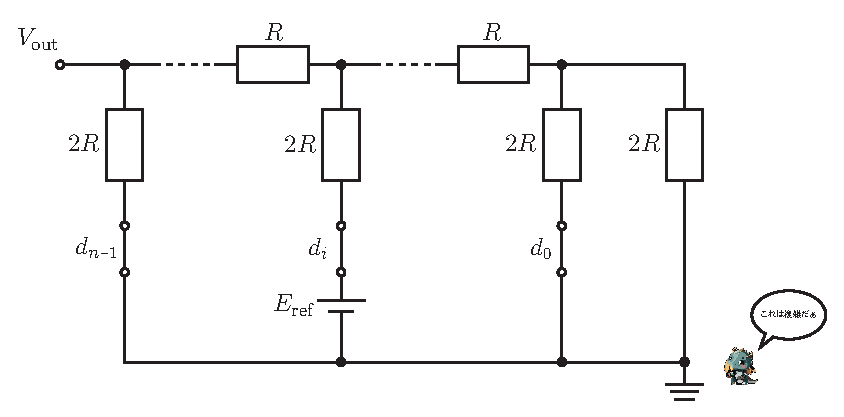
\includegraphics{figure1.eps}
  \vspace{10pt}\caption{ラダー回路の等価回路}
  \label{radder1}
\end{figure}\\
電気回路では重ね合わせの理が成り立つことから、$i$番目の電圧源のみを残しそれ以外の電圧源を短絡させたときの$V^i_\mathrm{out}$を求めることによって、最終的に求めたい$V_\mathrm{out}$はそれらの線形結合で表される($d_0,d_1,\cdots d_{n-1}$の全てが$0$のとき、$V_\mathrm{out}=0$となることは自明である)。図\ref{radder1}について$i$番目の電圧源のみを残し、それ以外を短絡させたあと、$0\ 〜\ i-1$番目の抵抗器を並列または直列で複数回合成することによって、図\ref{radder2}のようになり少し簡単になる。
\begin{figure}[h]
  \centering
  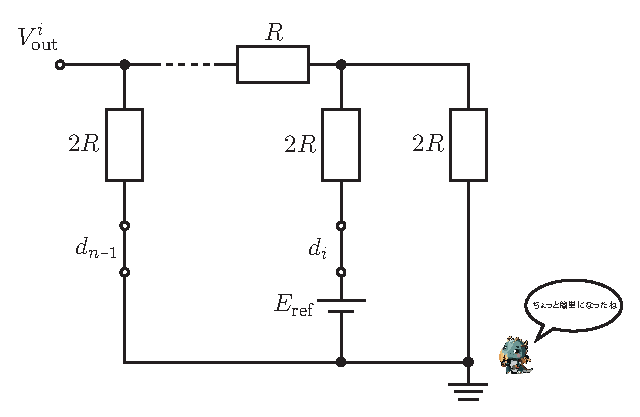
\includegraphics{figure2.eps}
  \vspace{10pt}\caption{ラダー回路の等価回路}
  \label{radder2}
\end{figure}\\
ここで、電圧源を電流源を用いて表せば図\ref{radder3}のようにできる。
\clearpage
\begin{figure}[h]
  \centering
  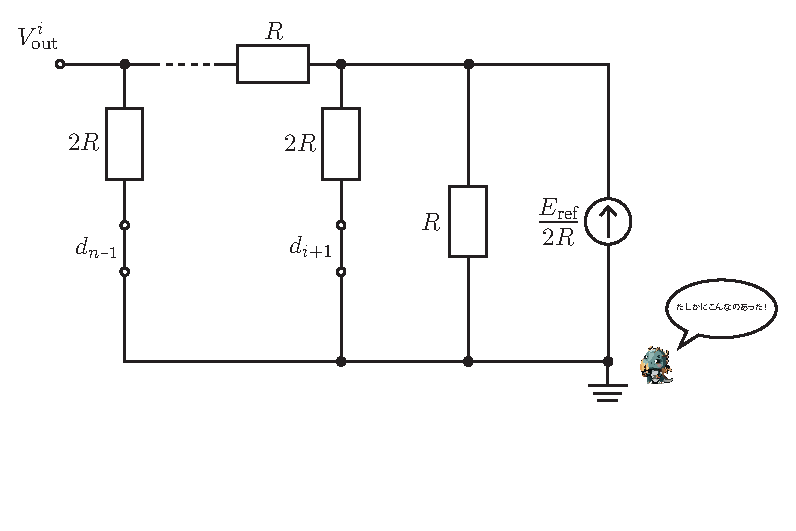
\includegraphics{figure3.eps}
  \vspace{-40pt}\caption{ラダー回路の等価回路}
  \label{radder3}
\end{figure}
先ほどの操作の逆を行うことによって図\ref{radder4}のようにできる。
\begin{figure}[h]
  \centering
  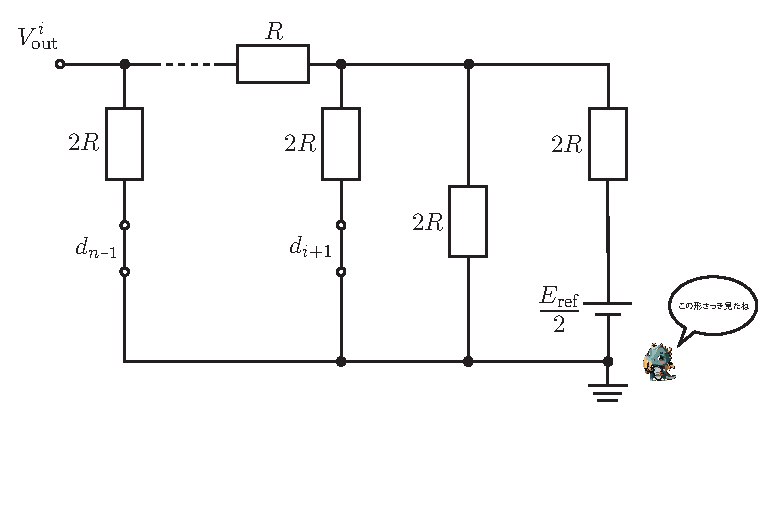
\includegraphics{figure4.eps}
  \vspace{-40pt}\caption{ラダー回路の等価回路}
  \label{radder4}
\end{figure}\\
図\ref{radder4}は図\ref{radder2}と同じ形をしていることがわかる。よって、同様の操作を繰り返すことによって図\ref{radder5}のようになる。
\clearpage
\begin{figure}[h]
  \centering
  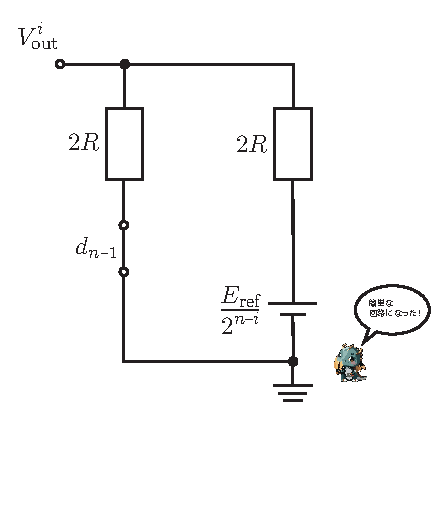
\includegraphics{figure5.eps}
  \vspace{-40pt}\caption{ラダー回路の等価回路}
  \label{radder5}
\end{figure}
図\ref{radder5}から$V^i_\mathrm{out}$を求めると
\begin{align}
  V^i_\mathrm{out}=\frac{1}{2^{n-i}}\frac{E_\mathrm{ref}}{2}
\end{align}
となる。よって、求めたい$V_\mathrm{out}$は(3)式の線形結合で表されるから、
\begin{align}
  V_\mathrm{out}=\sum^{n-1}_{i=0}2^{i-n}d_i\frac{E_\mathrm{ref}}{2}
\end{align}
となる。\\
\\
{\large \bfseries 3.2考察(f)について}\\
 マイクプリンアンプユニットとサンプルホールドユニットの間にLPFユニットを挿入する理由は、マイクから入力される信号にはノイズが多く存在するからである。普通、入力時に生じるノイズは私たちが扱いたいノイズよりも周波数がものすごく大きいことが多いためLPFユニットを用いる。また、もしLPFユニットを用いらなければノイズによって波形が大きく変化したときにサンプルホールドする場合が多くなり、サンプルホールド波形が入力波形と異なってしまう可能性が高まる。そのため、マイクプリンアンプユニットとサンプルホールドユニットの間にLPFユニットを挿入する。\\
\\
\hspace{-2pt}{\Large \bfseries 4.結論}\\
 デジタル信号の特徴を理解すると共に、アナログ信号のデジタル処理に必要なアナログ・デジタル変換の方法と性質を、実験を通じて理解することができた。\\
\\
{\Large \bfseries 参考文献}
\begin{thebibliography}{1}
\vspace{-1.5cm}
  \bibitem{text} D4実験テキスト.pdf 閲覧日:2023/12/19
  \bibitem{text1} D4実験\_補助資料2023v1.0.pdf 閲覧日:2023/12/19
  \bibitem{voice} 音の雑学大辞典,\ Pioneer\\(https:// jpn.pioneer/ja/carrozzeria/museum/oto/01\_a03.html)閲覧日:2023/12/19
\end{thebibliography}
\clearpage
$============================================================$\\
学籍番号:62115799\\
 氏  名 :平井優我\\
$============================================================$\\
■自己評価点 (100点満点): 100点 〔最低希望点: 100点〕\\
・このように評価する理由:\\自分で書いたレポートは100点じゃないとおかしい。



$------------------------------------------------------------$\\
■レポートで特に力を入れたところ:\\
全体。


$------------------------------------------------------------$\\
■レポートで難しかった・わからなかったところ:\\
なし。


$------------------------------------------------------------$\\
■レポートについて質問・確認したいこと:\\
なし。


$------------------------------------------------------------$\\
■その他の質問・意見・要望など:\\
ヘッドホンで聞いている高音質ってすごいんだなと思った。
\end{document}
